%%%%%%%%%%%%%%%%%%%%%%%%%%%%%%%%%%%%%%%%%%%%%%%%%%%%%%%%%%%%%%%%%%%%%%
% Overleaf (WriteLaTeX) Example: Molecular Chemistry Presentation
%
% Source: http://www.overleaf.com
%
% In these slides we show how Overleaf can be used with standard 
% chemistry packages to easily create professional presentations.
% 
% Feel free to distribute this example, but please keep the referral
% to overleaf.com
% 
%%%%%%%%%%%%%%%%%%%%%%%%%%%%%%%%%%%%%%%%%%%%%%%%%%%%%%%%%%%%%%%%%%%%%%

\documentclass{beamer}

\mode<presentation>
{
  \usetheme{Madrid}       % or try default, Darmstadt, Warsaw, ...
  \usecolortheme{default} % or try albatross, beaver, crane, ...
  \usefonttheme{default}    % or try default, structurebold, ...
  \setbeamertemplate{navigation symbols}{}
  \setbeamertemplate{caption}[numbered]
} 

\usepackage[english]{babel}
\usepackage[utf8x]{inputenc}
\usepackage{graphicx}
\usepackage{hyperref}
  \hypersetup{colorlinks=true}
  \hypersetup{urlcolor=blue}
  \hypersetup{linkcolor = .}
\usepackage{xcolor}
\usepackage{siunitx}
  \sisetup{separate-uncertainty = true}
\usepackage{physics}
\usepackage[font=small,labelfont=bf]{caption}
\usepackage{subcaption}
\usepackage[en-GB]{datetime2}
\usepackage{overpic}
\usepackage{feynmp}
\DeclareGraphicsRule{*}{mps}{*}{}
\usepackage{scalerel}
\newcommand{\mylbrace}[2]{\vspace{#2pt}\hspace{6pt}\scaleleftright[\dimexpr5pt+#1\dimexpr0.06pt]{\lbrace}{\rule[\dimexpr2pt-#1\dimexpr0.5pt]{-4pt}{#1pt}}{.}}
\newcommand{\myrbrace}[2]{\vspace{#2pt}\scaleleftright[\dimexpr5pt+#1\dimexpr0.06pt]{.}{\rule[\dimexpr2pt-#1\dimexpr0.5pt]{-4pt}{#1pt}}{\rbrace}\hspace{6pt}}

% Here's where the presentation starts, with the info for the title slide
\title[TORCH meeting]{PID studies with proto-TORCH testbeam \\TORCH meeting}

\author{Martin Tat}
\institute{University of Oxford}
\date{7th April 2022}

\titlegraphic{
\includegraphics[height = 2cm]{lhcb.jpg}\hspace{2cm}~%
              
\includegraphics[height = 2cm]{OxfordLogo.pdf}}

\begin{document}

\begin{frame}
  \titlepage
\end{frame}

% These three lines create an automatically generated table of contents.
%\begin{frame}{Outline}
%  \tableofcontents
%\end{frame}

\section{Introduction}
\begin{frame}{Introduction}
  \begin{itemize}
    \setlength\itemsep{2.0em}
    \item{My work so far:}
    \begin{itemize}
    \setlength\itemsep{0.5em}
      \item{Study how photons are propagated through TORCH optics}
      \item{Study analytical photon reconstruction from MCP hits}
      \item{Understand likelihood calculation}
    \end{itemize}
    \item{Long term goal:}
    \begin{itemize}
    \setlength\itemsep{0.5em}
      \item{Build on Jenny's testbeam data analysis:}
      \begin{itemize}
        \item{Jenny has focused on timing resolution studies}
        \item{I will study PID separation power}
      \end{itemize}
      \item{Prepare for PID study of next testbeam data}
    \end{itemize}
    \item{Thanks to:}
    \begin{itemize}
      \item{Thomas Blake for providing code}
      \item{Jenny for providing testbeam data}
    \end{itemize}
  \end{itemize}
\end{frame}

\section{Introduction to reconstruction code}
\begin{frame}{Introduction to reconstruction code}
  \begin{itemize}
    \item{Forwards propagation:}
    \begin{enumerate}
      \item{Trace emitted photon through quartz bar}
      \item{Reflect in cylindrical mirror}
      \item{MCP hit!}
    \end{enumerate}
  \end{itemize}
  \begin{figure}
    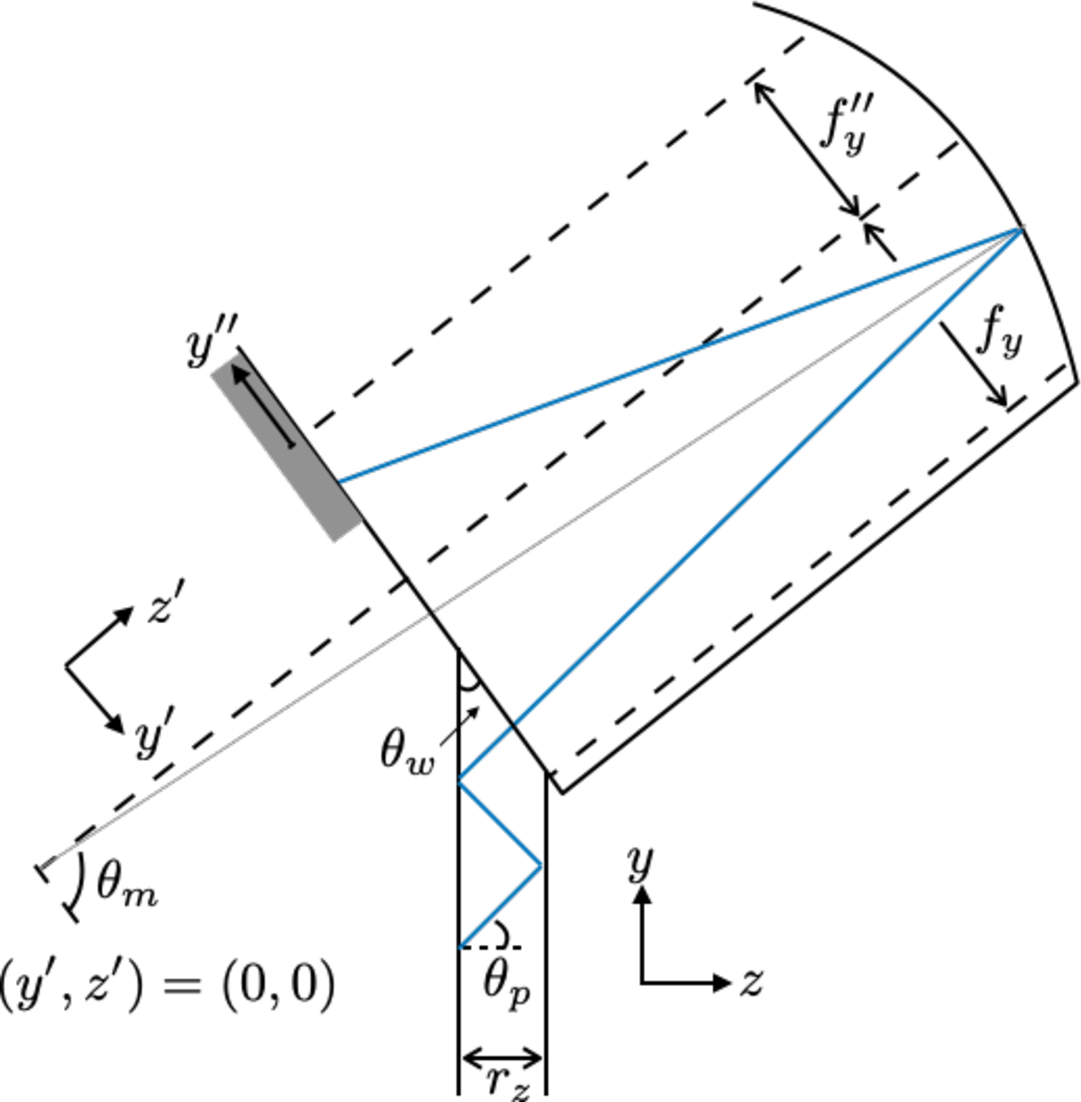
\includegraphics[width = 0.35\textwidth]{Plots/torch-geometry.pdf}
  \end{figure}
  \begin{itemize}
    \item{Reconstruction and PID algorithm described in \href{https://www.overleaf.com/project/5d0b9c5a5005405666aacd05}{LHCb-PUB-2022-007}}
  \end{itemize}
\end{frame}

\begin{frame}{Introduction to reconstruction code}
  \begin{itemize}
    \item{Reconstruction:}
    \begin{enumerate}
      \item{Reconstruct photon direction from vertical MCP pixel position}
      \item{From photon direction, calculate $\theta_c\to n_{\rm phase}\to n_{\rm group}$}
      \item{Reconstruct propagation time!}
    \end{enumerate}
  \end{itemize}
  \begin{figure}
    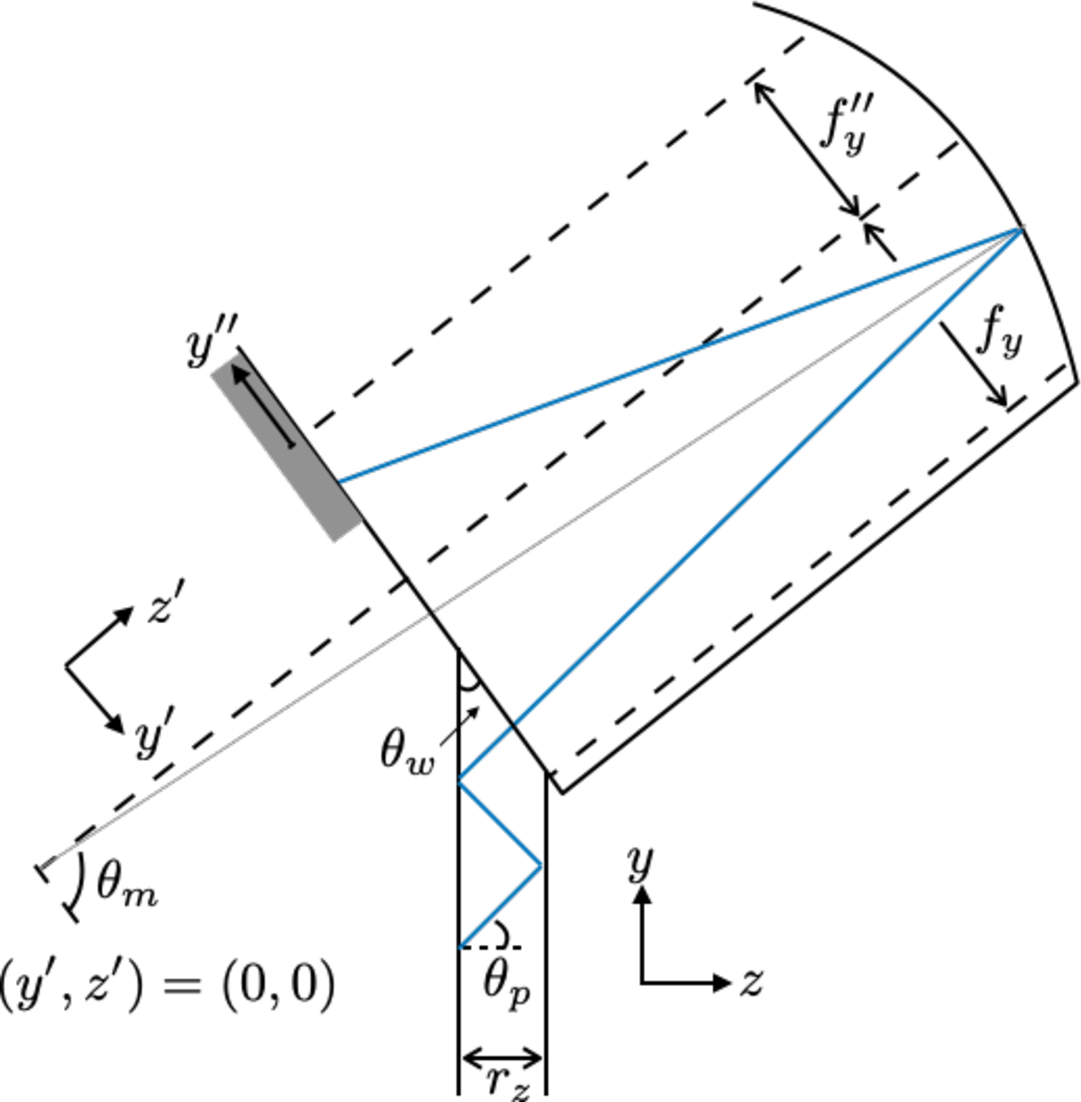
\includegraphics[width = 0.35\textwidth]{Plots/torch-geometry.pdf}
  \end{figure}
  \begin{itemize}
    \item{Reconstruction described in \href{https://www.overleaf.com/project/5d0b9c5a5005405666aacd05}{LHCb-PUB-2022-007}}
  \end{itemize}
\end{frame}

\section{Hit maps}
\begin{frame}{Hit maps}
  \begin{figure}
    \centering
    \vspace{-0.2cm}
    \begin{subfigure}{0.5\textwidth}
      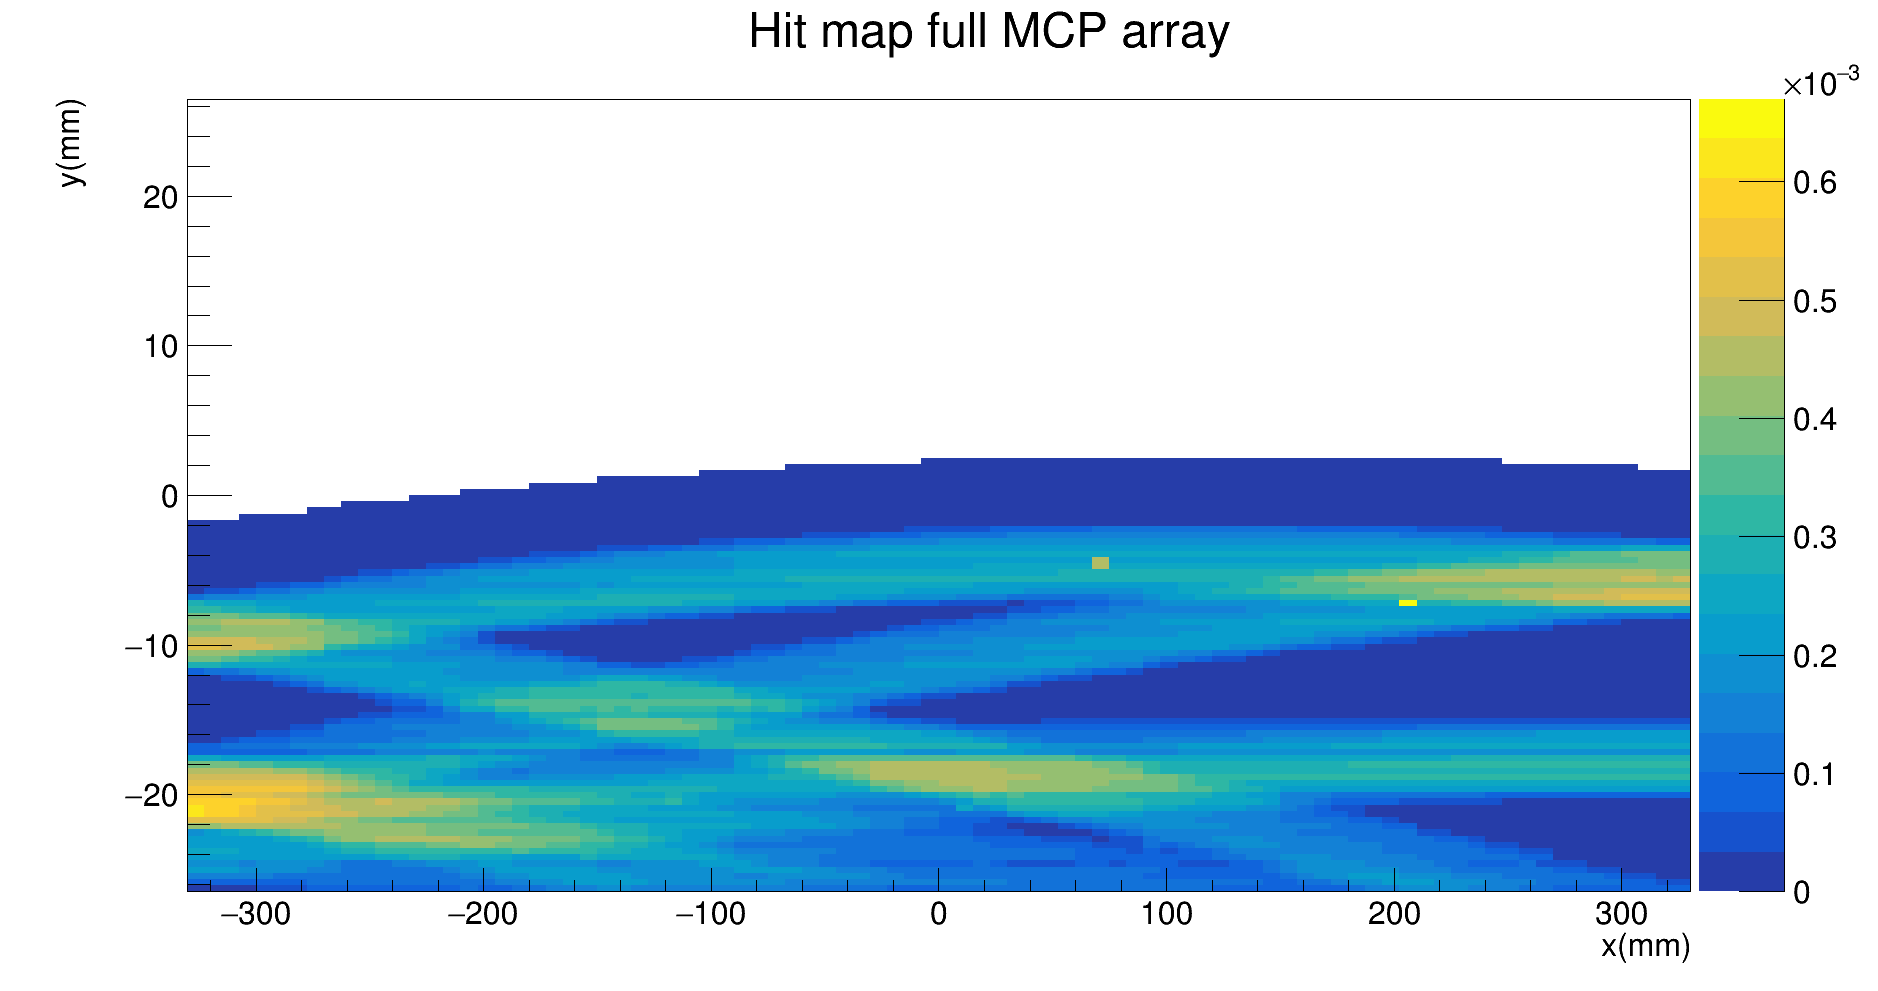
\includegraphics[width = 1.0\textwidth]{Plots/HitMapMCPFullMiddle.png}
      \caption{Full MCP array}
    \end{subfigure}%
    \begin{subfigure}{0.5\textwidth}
      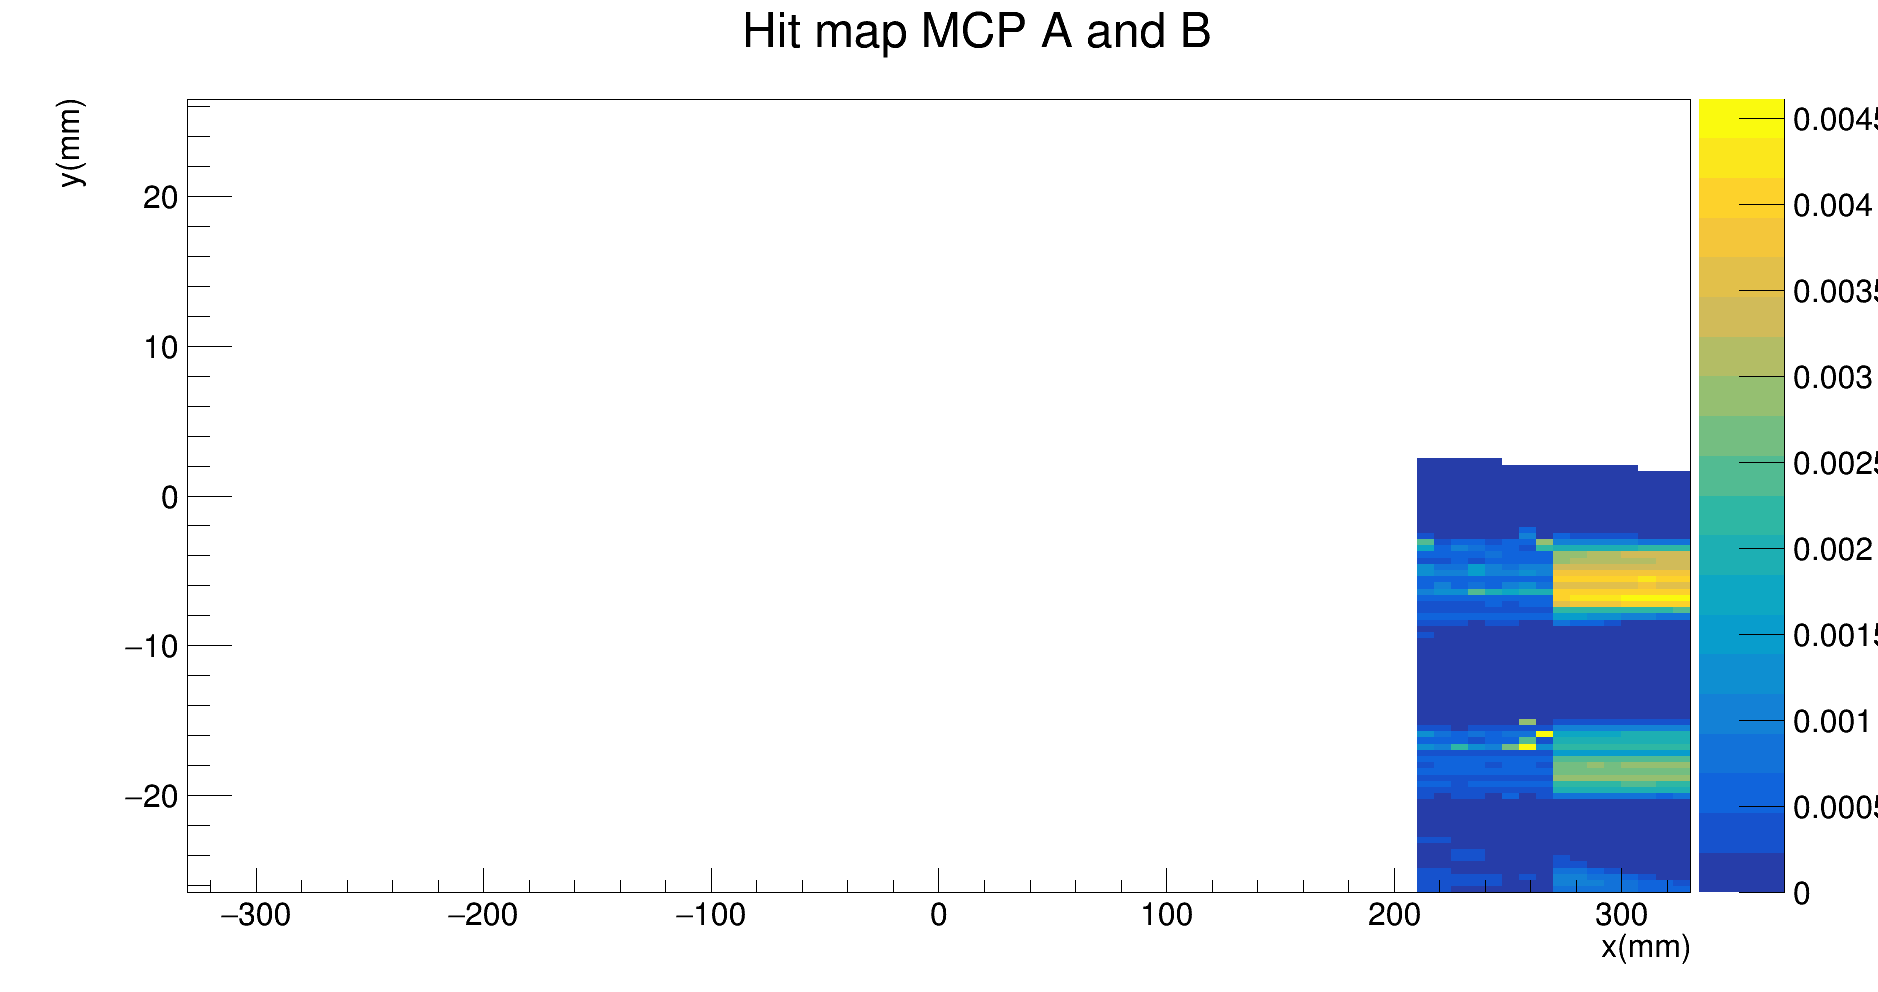
\includegraphics[width = 1.0\textwidth]{Plots/HitMapMCPABMiddle.png}
      \caption{MCP A and B}
    \end{subfigure}
    \caption{Track incident $\SI{1}{\meter}$ from top}
  \end{figure}
\end{frame}

\begin{frame}{Hit maps}
  \begin{figure}
    \centering
    \vspace{-0.2cm}
    \begin{subfigure}{0.5\textwidth}
      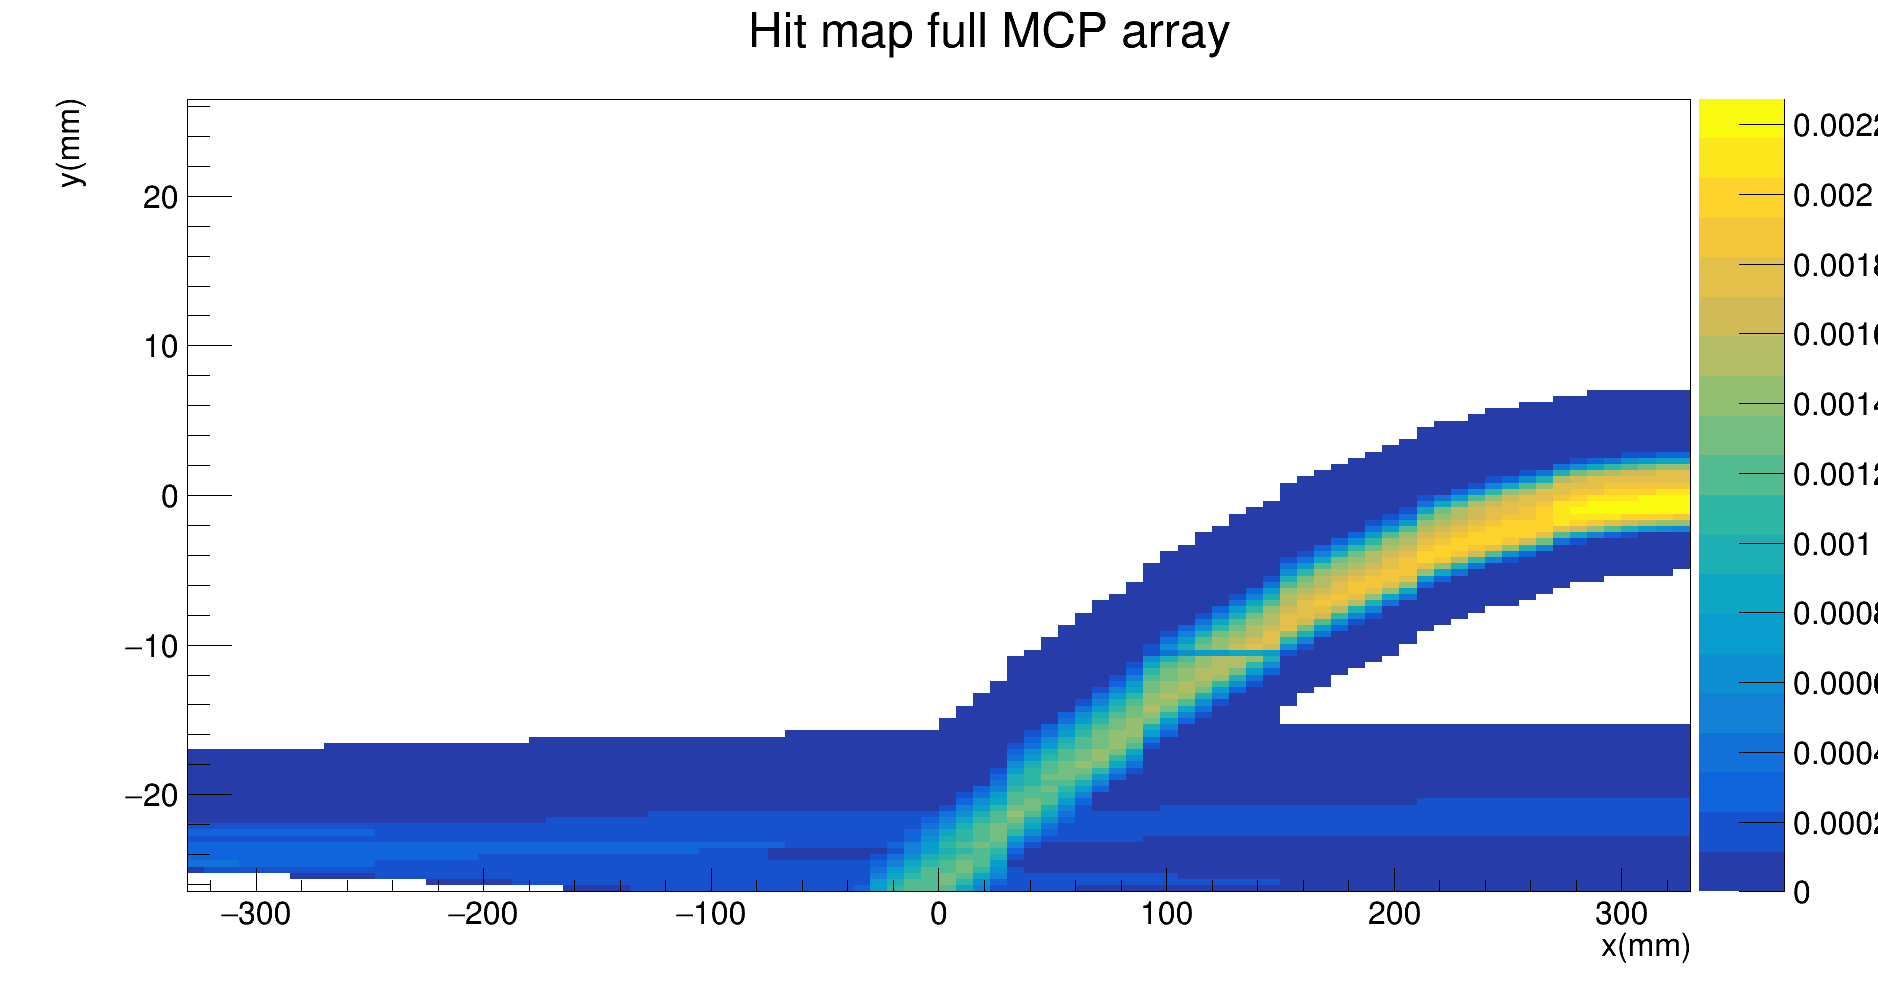
\includegraphics[width = 1.0\textwidth]{Plots/HitMapMCPFull.png}
      \caption{Full MCP array}
    \end{subfigure}%
    \begin{subfigure}{0.5\textwidth}
      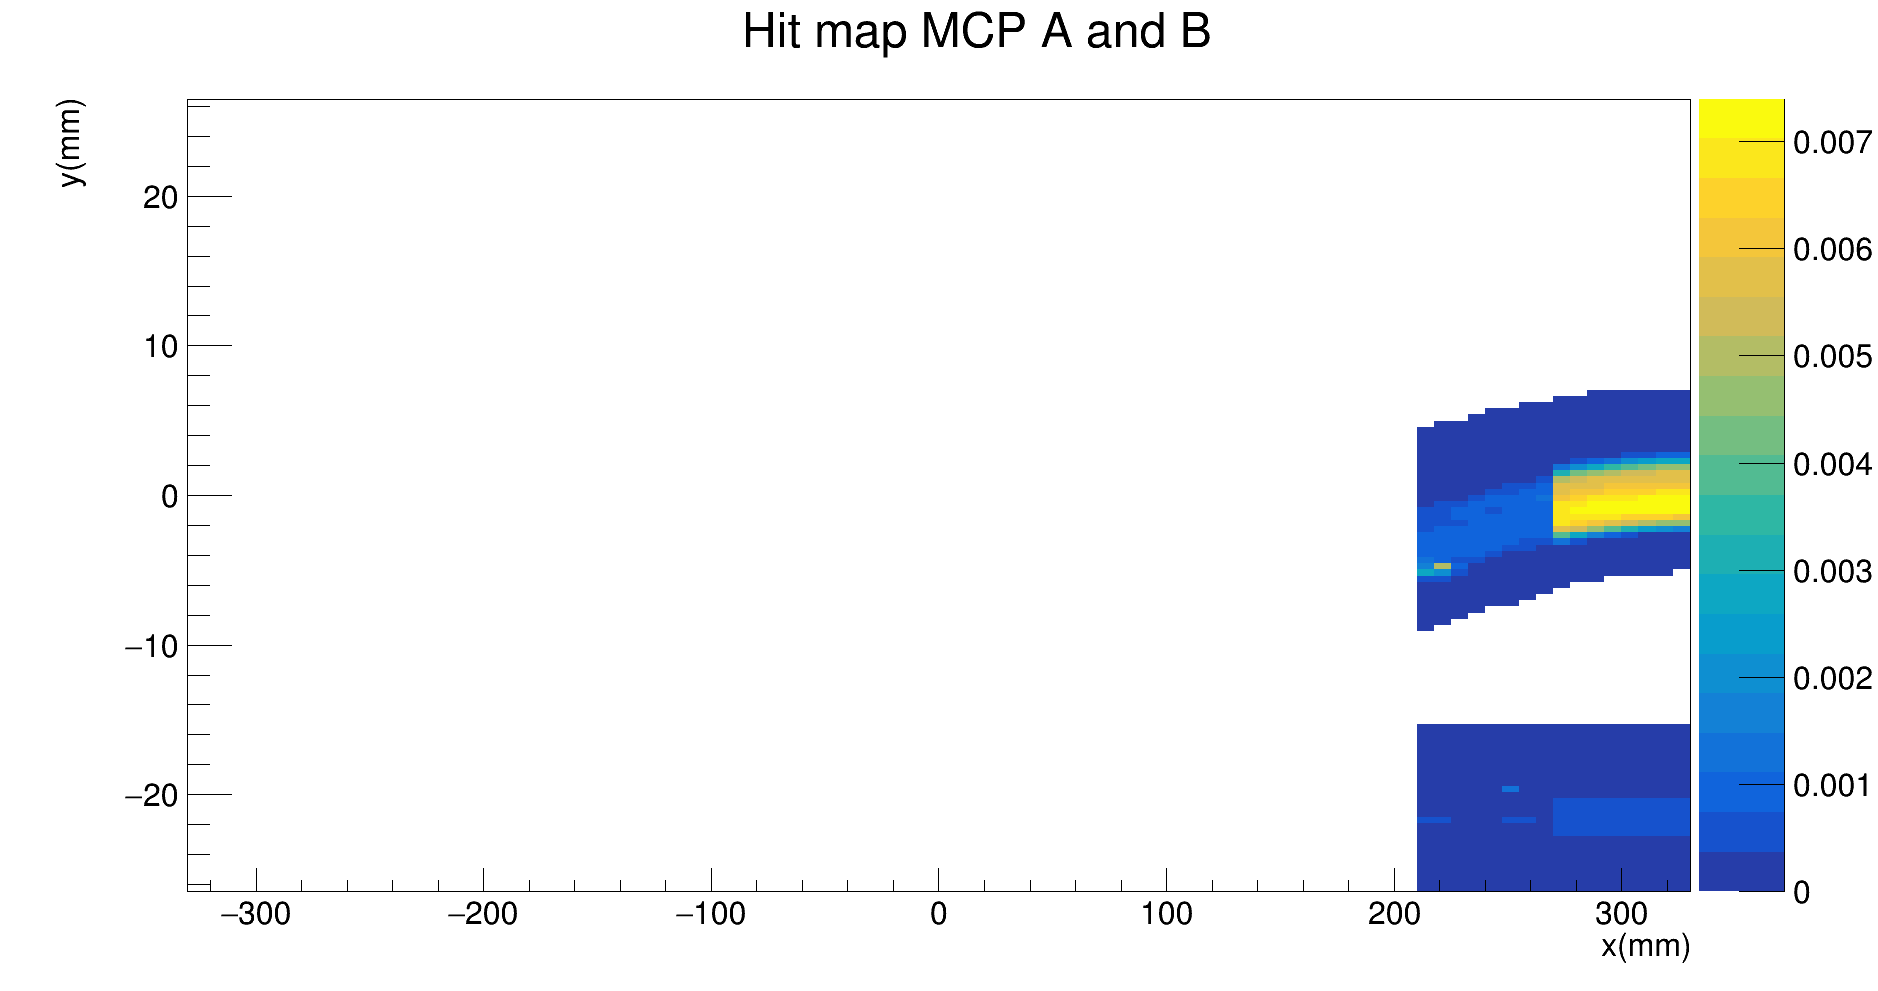
\includegraphics[width = 1.0\textwidth]{Plots/HitMapMCPAB.png}
      \caption{MCP A and B}
    \end{subfigure}
    \caption{Track incident on top right corner (position 1)}
  \end{figure}
\end{frame}

\section{Likelihood calculation}
\begin{frame}{Likelihood calculation}
  \begin{itemize}
    \item{Probability of photon hit with energy $E_\gamma$, azimuthal angle $\phi_c$, time $t_0$:}
  \end{itemize}
  \begin{align*}
    P(E_\gamma, \phi_c, z, t_0) =& P(\phi_c)P(z)P(t_0)P(E_\gamma)\Theta(E_\gamma, \phi_c, z) \\
    =& \frac{1}{2\pi}\frac{1}{r_z}P(E_\gamma)P(t_0)\Theta(E_\gamma, \phi_c, z)
  \end{align*}
  \begin{itemize}
    \item{Transform to detector coordinates $(x_d, y_d)$:}
  \end{itemize}
  \begin{equation*}
    P(x_d, y_d, t_d) = P(E_\gamma, \phi_c, t_0)/\lvert J\rvert, \quad \lvert J\rvert = \Big\lvert\frac{\partial y_d}{\partial E_\gamma}\frac{\partial x_d}{\partial\phi_c} - \frac{\partial x_d}{\partial E_\gamma}\frac{\partial y_d}{\partial\phi_c}\Big\rvert
  \end{equation*}
  \begin{itemize}
    \item{$P(t_0)$: Gaussian PDF with $\sim\SI{70}{\pico\second}$ time resolution}
    \item{$P(E_\gamma)$: Frank-Tamm formula}
  \end{itemize}
  \begin{itemize}
    \item{PID algorithm described in \href{https://www.overleaf.com/project/5d0b9c5a5005405666aacd05}{LHCb-PUB-2022-007}}
  \end{itemize}
\end{frame}

\begin{frame}{Test likelihood calculation}
  \begin{itemize}
    \setlength\itemsep{1.5em}
    \item{Does it work?}
    \item{Set up single charged track simulation:}
    \begin{enumerate}
      \setlength\itemsep{0.8em}
      \item{Send single particle (pion, kaon, proton) through quartz}
      \item{Generate Cherenkov photons}
      \item{Propagate photons to MCPs}
      \item{Calculate likelihood from photon hits}
      \item{Start over from step 1}
    \end{enumerate}
    \item{No background hypothesis}
    \item{Turn on pixelisation, charge sharing, clustering}
  \end{itemize}
\end{frame}

\section{Likelihood simulations}
\begin{frame}{Pion-Proton likelihood simulations}
  \begin{figure}
    \centering
    \vspace{-0.2cm}
    \begin{subfigure}{0.5\textwidth}
      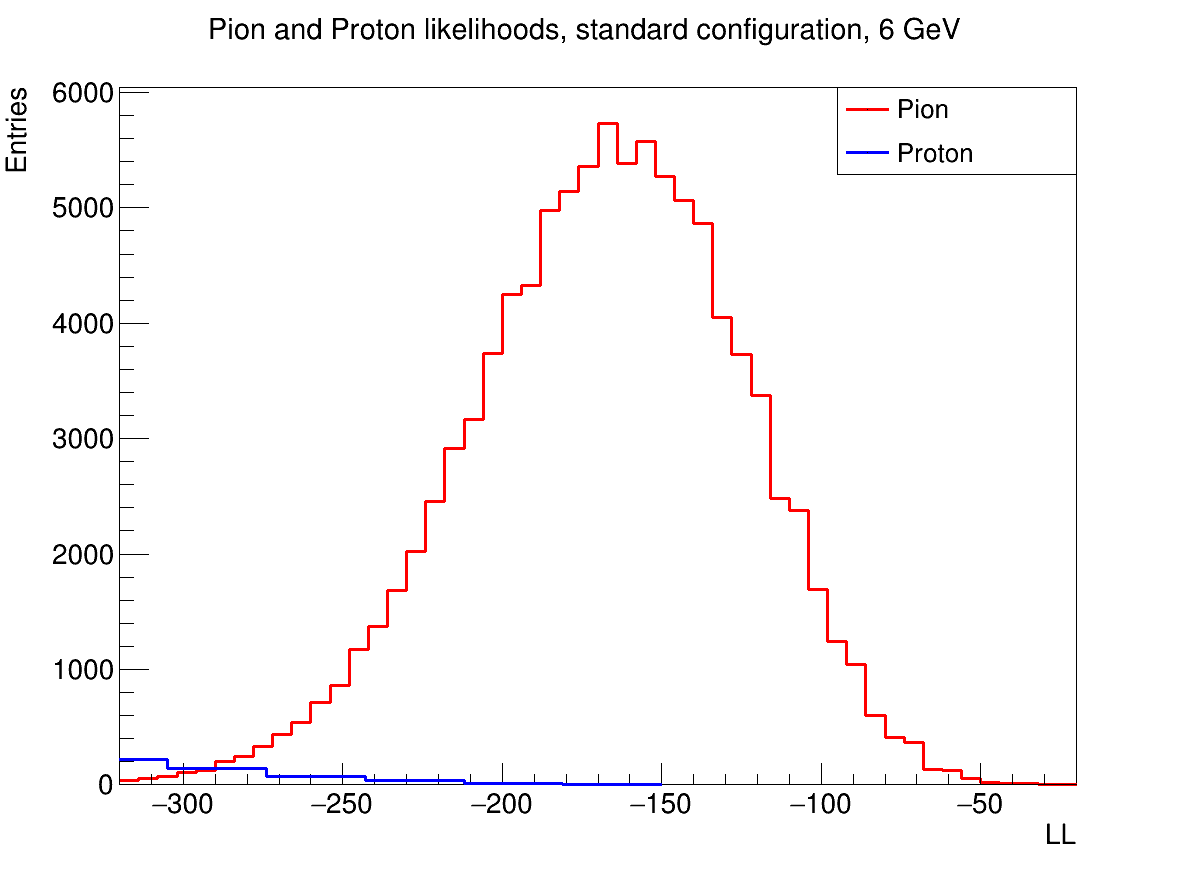
\includegraphics[width = 1.0\textwidth]{Plots/ProtonPionLL6GeVStandard.png}
      \caption{Pion and proton hypotheses}
    \end{subfigure}%
    \begin{subfigure}{0.5\textwidth}
      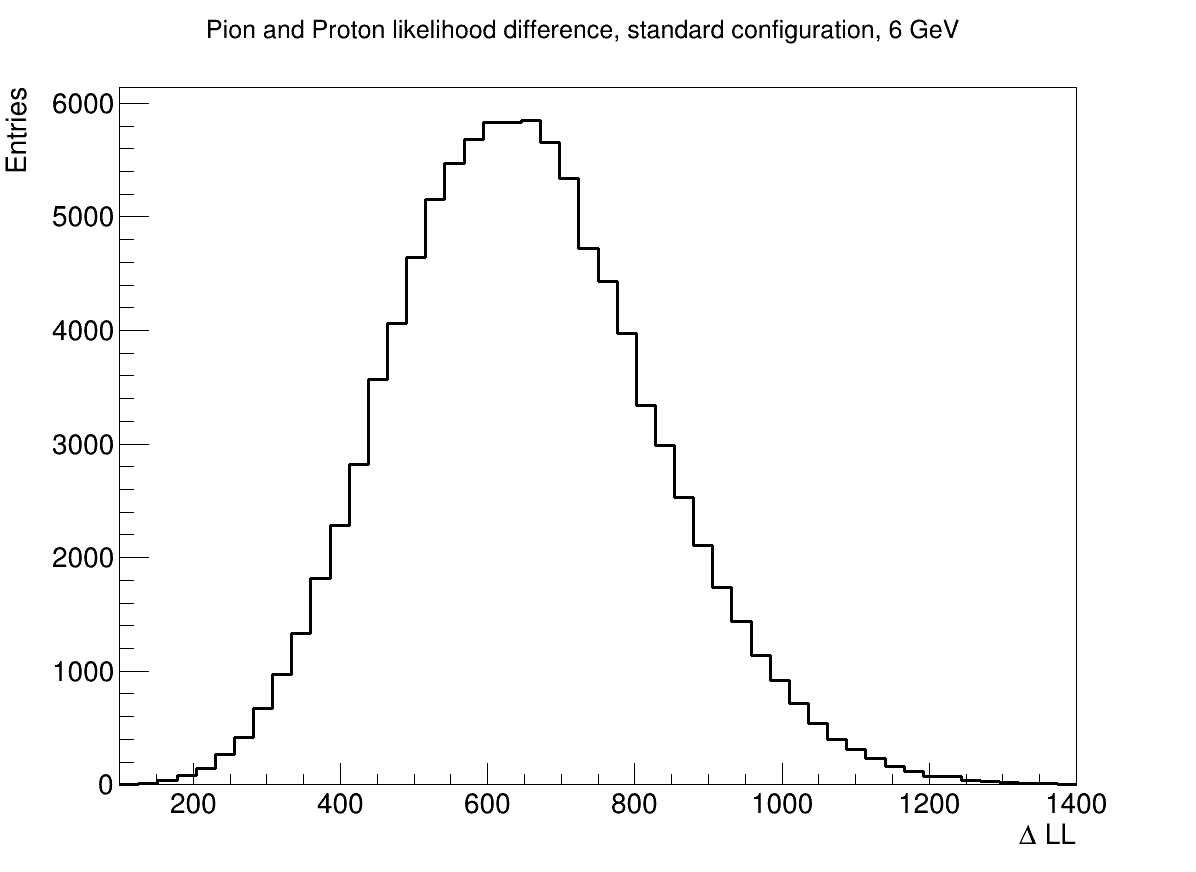
\includegraphics[width = 1.0\textwidth]{Plots/ProtonPionDLL6GeVStandard.png}
      \caption{Pion-proton $\Delta{\rm LL}$}
    \end{subfigure}
    \caption{Log likelihood at $\SI{6}{\giga\eV}$}
  \end{figure}
\end{frame}

\begin{frame}{Pion-Proton likelihood simulations}
  \begin{figure}
    \centering
    \vspace{-0.2cm}
    \begin{subfigure}{0.5\textwidth}
      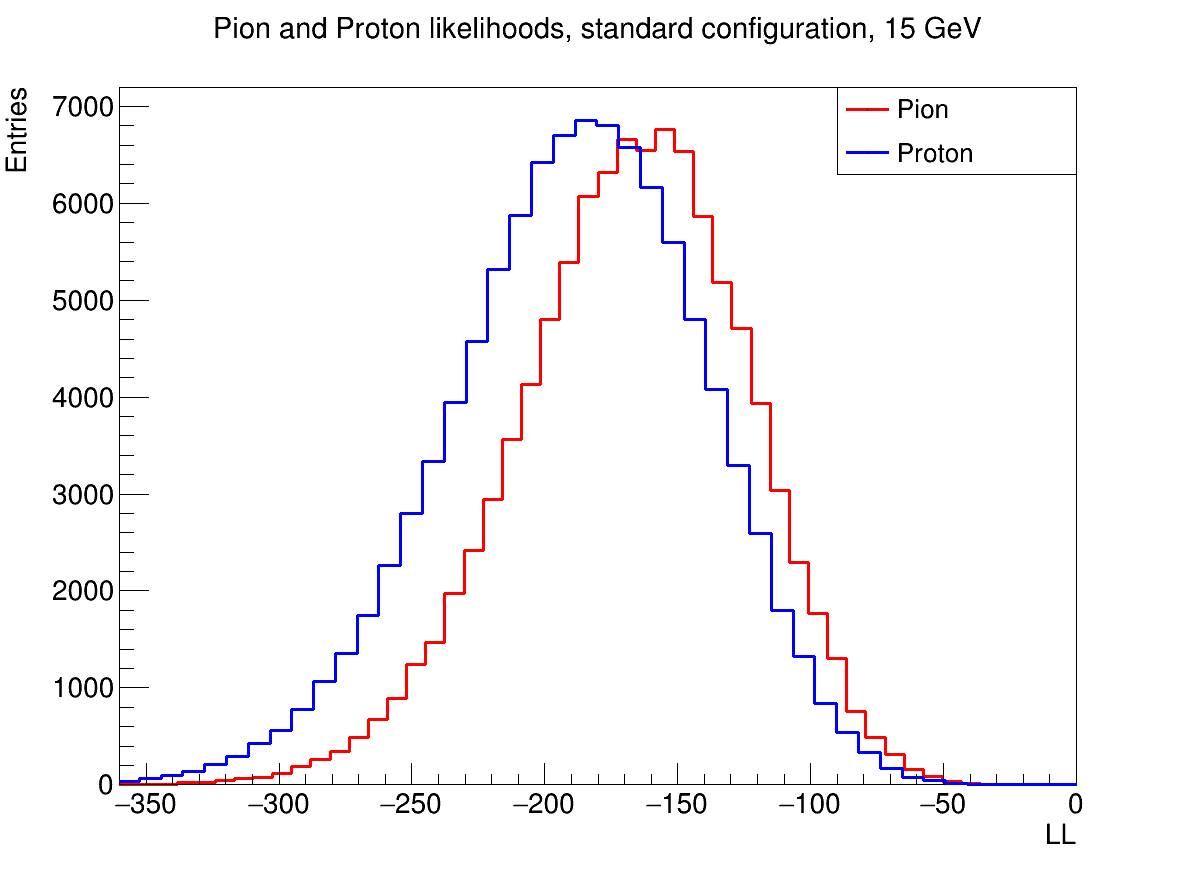
\includegraphics[width = 1.0\textwidth]{Plots/ProtonPionLL15GeVStandard.png}
      \caption{Pion and proton hypotheses}
    \end{subfigure}%
    \begin{subfigure}{0.5\textwidth}
      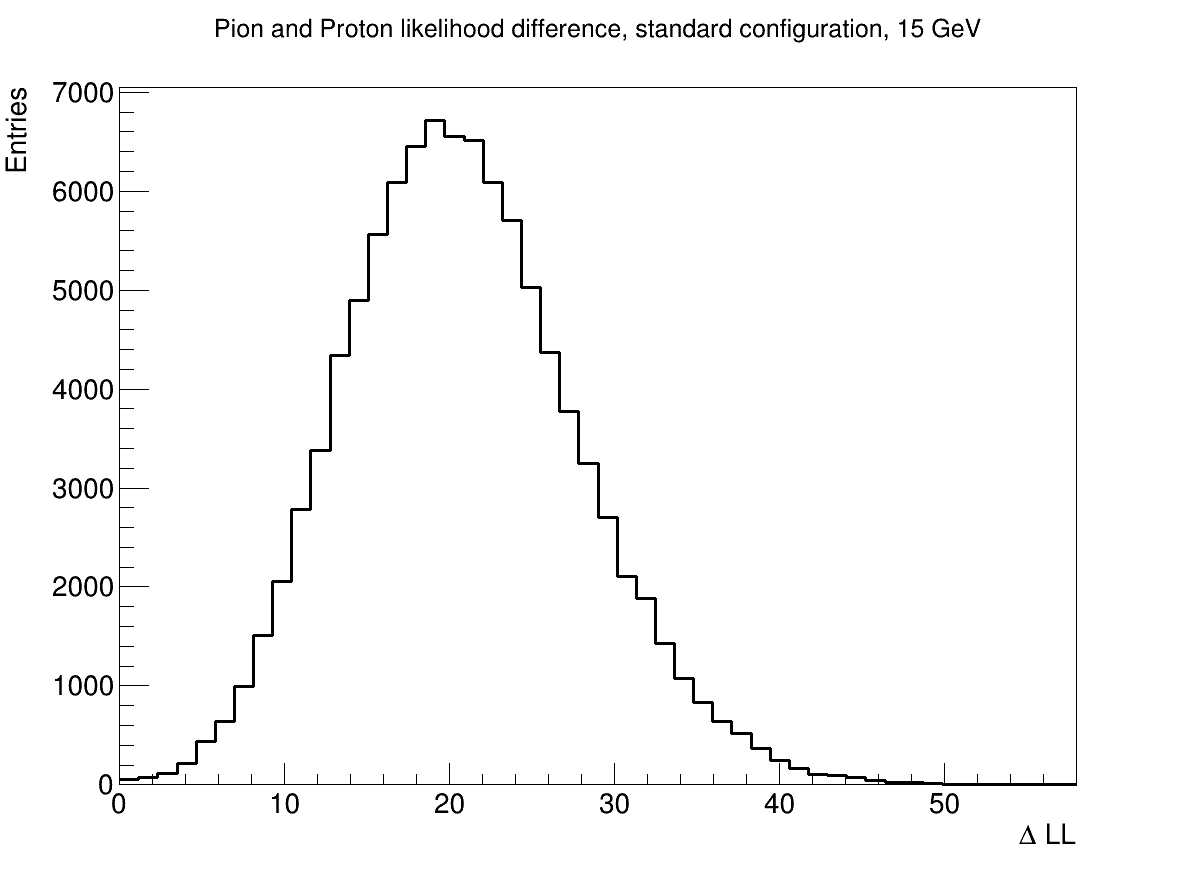
\includegraphics[width = 1.0\textwidth]{Plots/ProtonPionDLL15GeVStandard.png}
      \caption{Pion-proton $\Delta{\rm LL}$}
    \end{subfigure}
    \caption{Log likelihood at $\SI{15}{\giga\eV}$}
  \end{figure}
\end{frame}

\begin{frame}{Pion-Proton likelihood simulations}
  \begin{figure}
    \centering
    \vspace{-0.2cm}
    \begin{subfigure}{0.5\textwidth}
      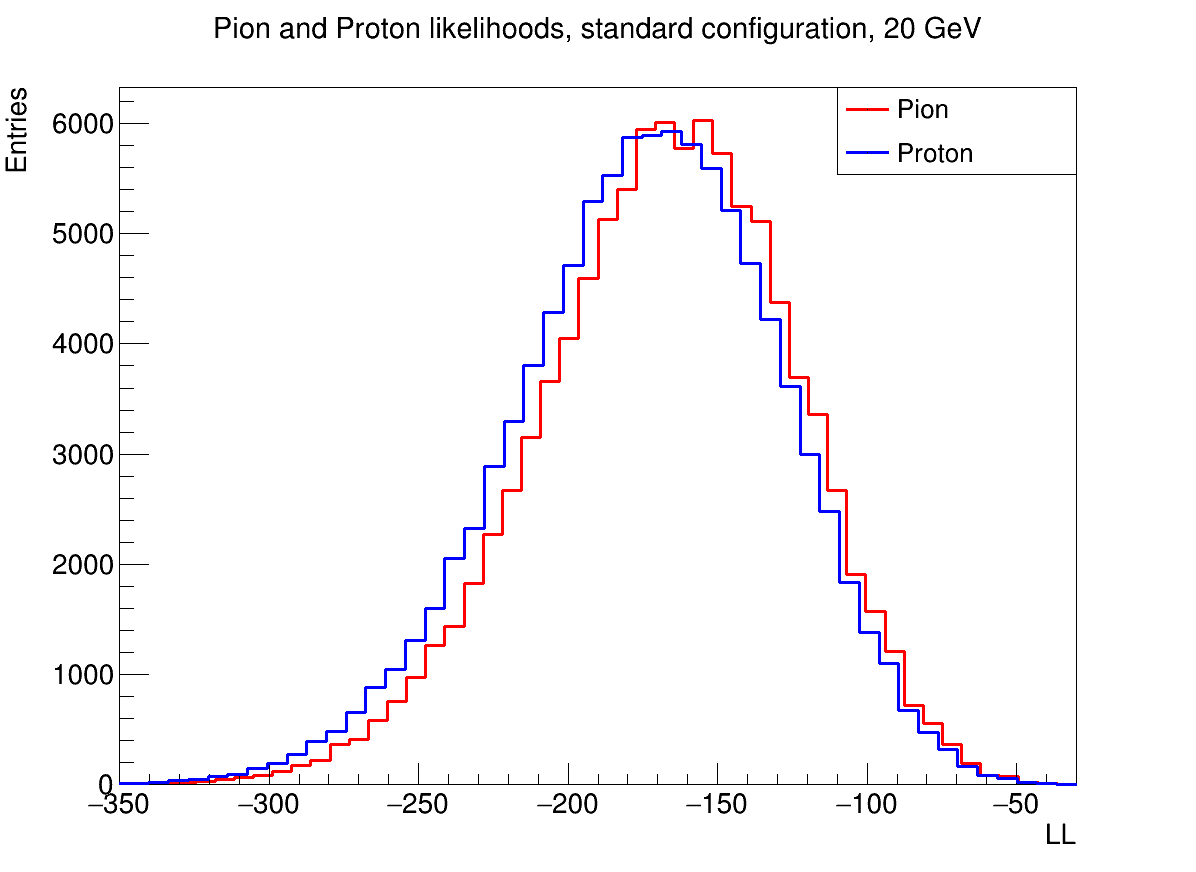
\includegraphics[width = 1.0\textwidth]{Plots/ProtonPionLL20GeVStandard.png}
      \caption{Pion and proton hypotheses}
    \end{subfigure}%
    \begin{subfigure}{0.5\textwidth}
      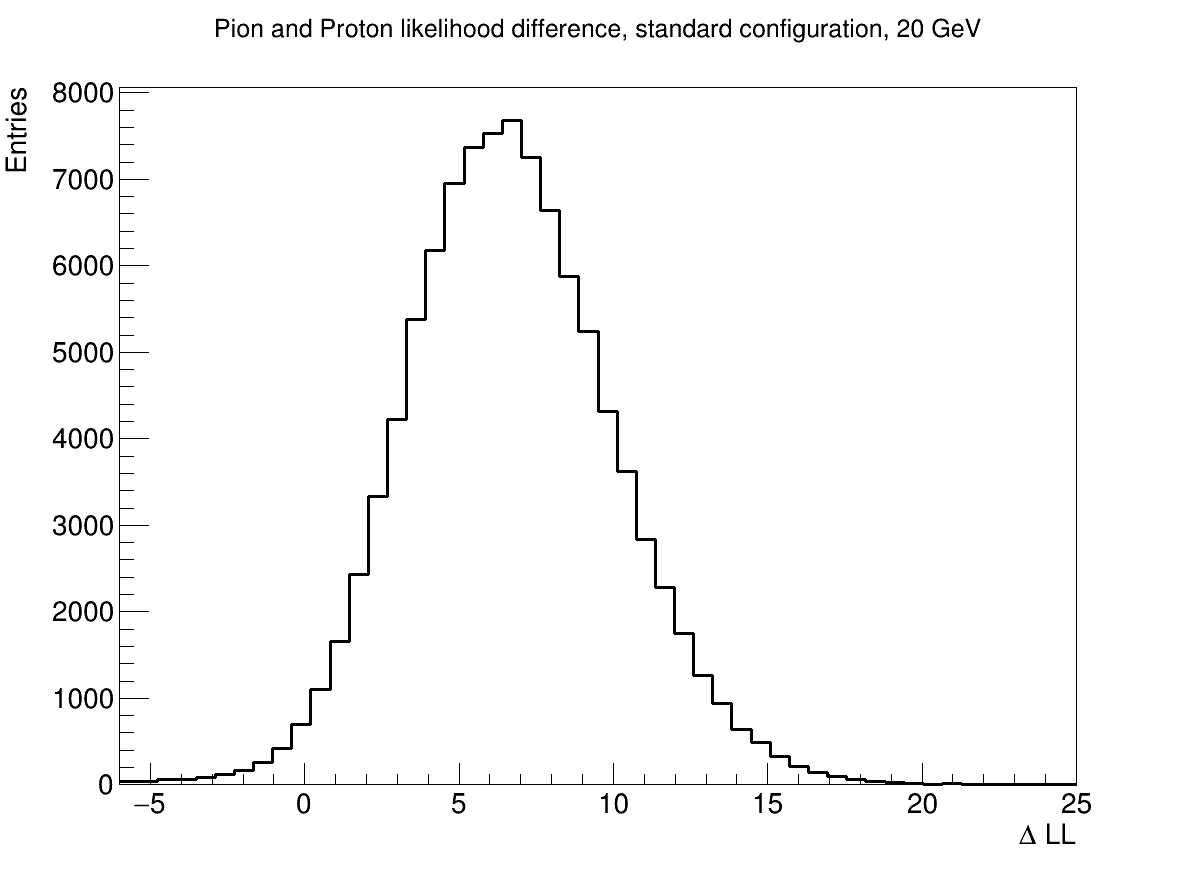
\includegraphics[width = 1.0\textwidth]{Plots/ProtonPionDLL20GeVStandard.png}
      \caption{Pion-proton $\Delta{\rm LL}$}
    \end{subfigure}
    \caption{Log likelihood at $\SI{20}{\giga\eV}$}
  \end{figure}
\end{frame}

\begin{frame}{Pion-Kaon likelihood simulations}
  \begin{figure}
    \centering
    \vspace{-0.2cm}
    \begin{subfigure}{0.5\textwidth}
      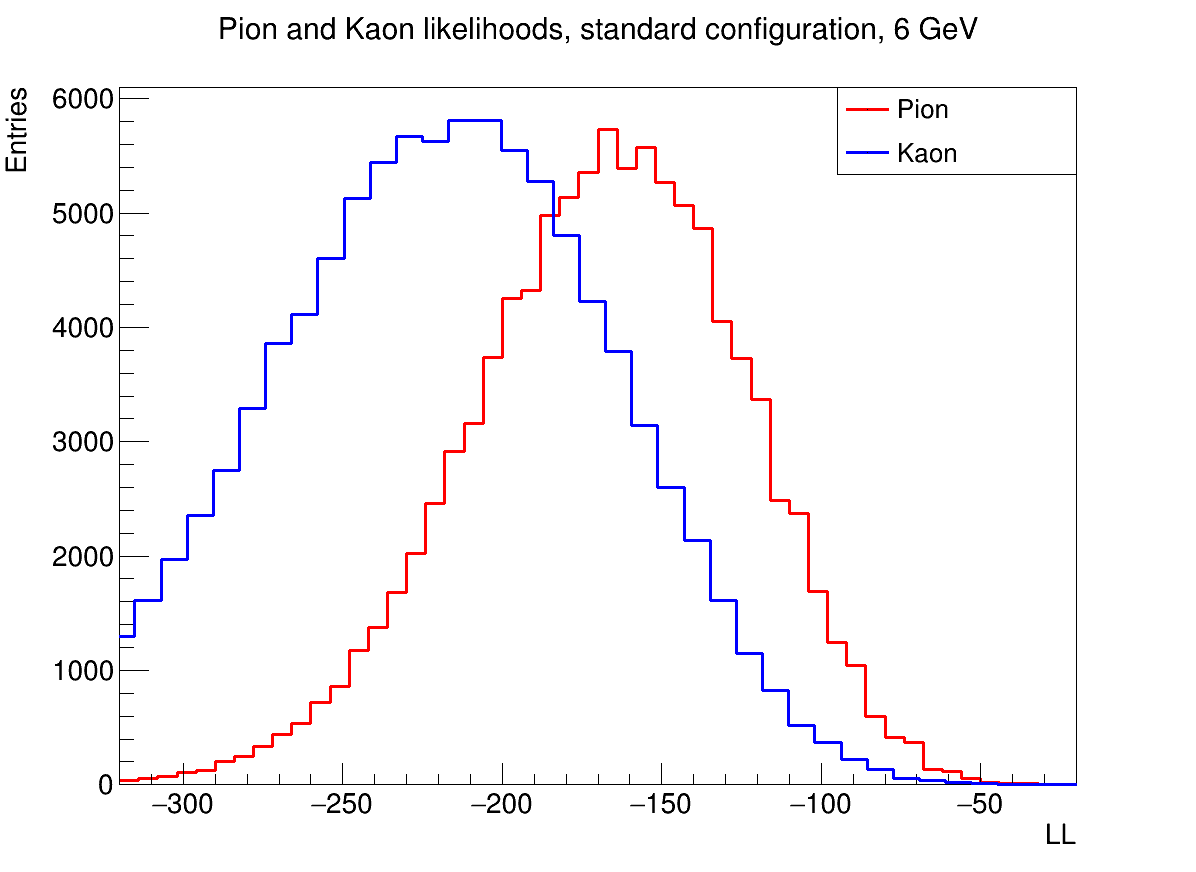
\includegraphics[width = 1.0\textwidth]{Plots/PionKaonLL6GeVStandard.png}
      \caption{Pion and kaon hypotheses}
    \end{subfigure}%
    \begin{subfigure}{0.5\textwidth}
      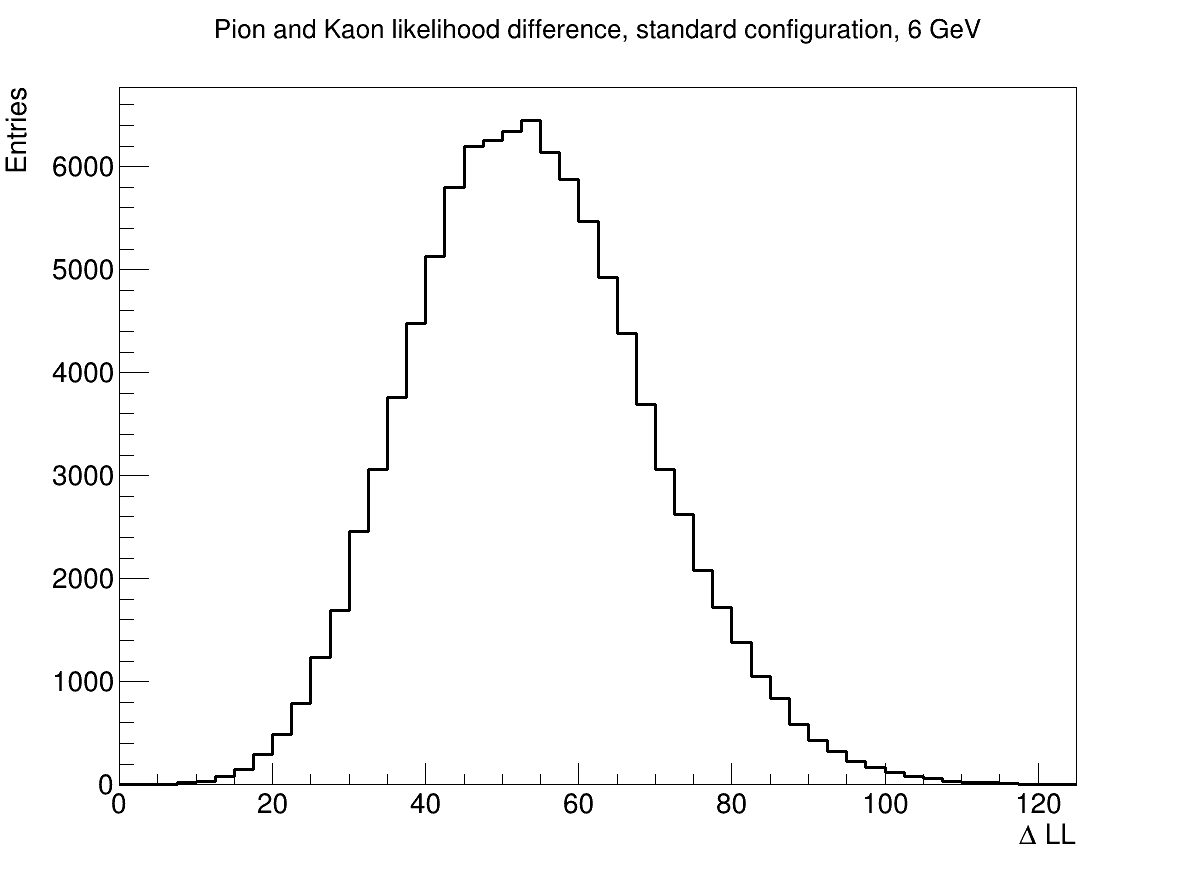
\includegraphics[width = 1.0\textwidth]{Plots/PionKaonDLL6GeVStandard.png}
      \caption{Pion-kaon $\Delta{\rm LL}$}
    \end{subfigure}
    \caption{Log likelihood at $\SI{6}{\giga\eV}$}
  \end{figure}
\end{frame}

\begin{frame}{Pion-Kaon likelihood simulations}
  \begin{figure}
    \centering
    \vspace{-0.2cm}
    \begin{subfigure}{0.5\textwidth}
      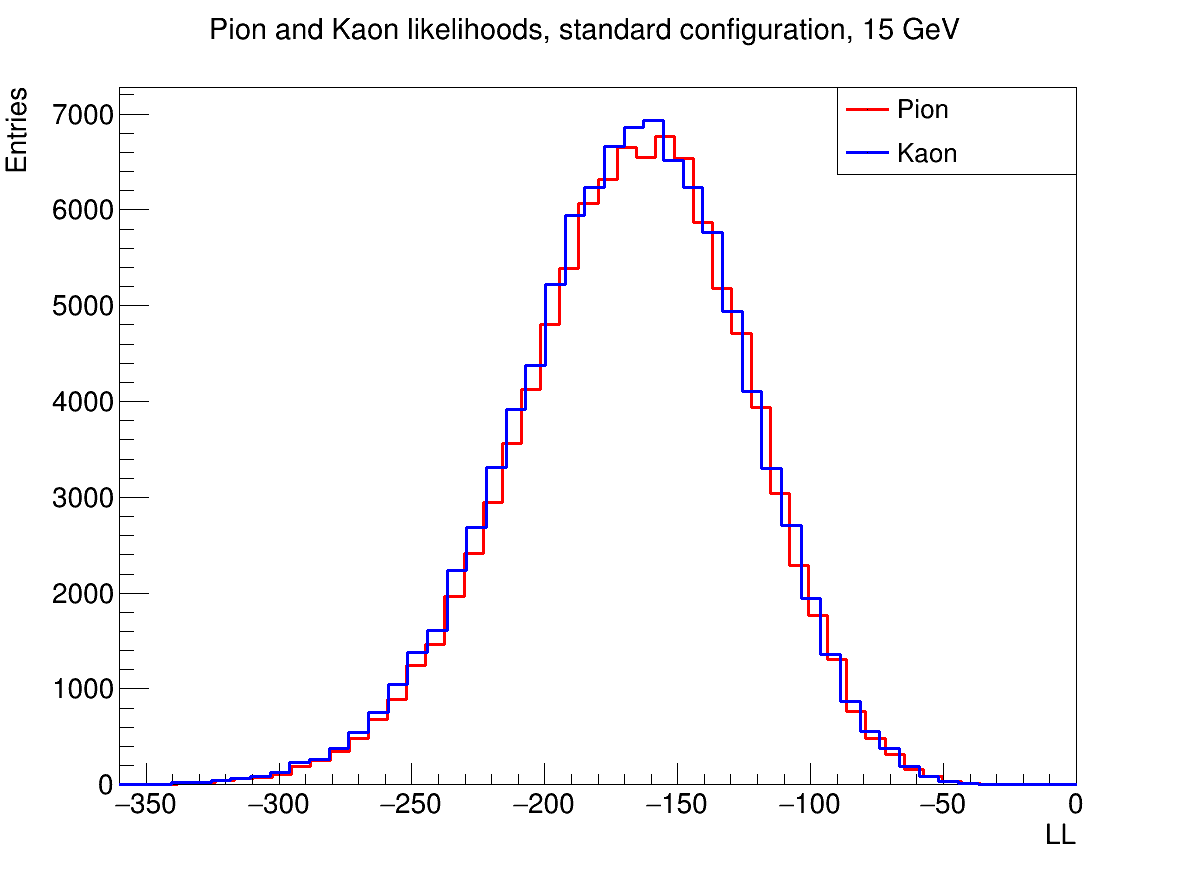
\includegraphics[width = 1.0\textwidth]{Plots/PionKaonLL15GeVStandard.png}
      \caption{Pion and kaon hypotheses}
    \end{subfigure}%
    \begin{subfigure}{0.5\textwidth}
      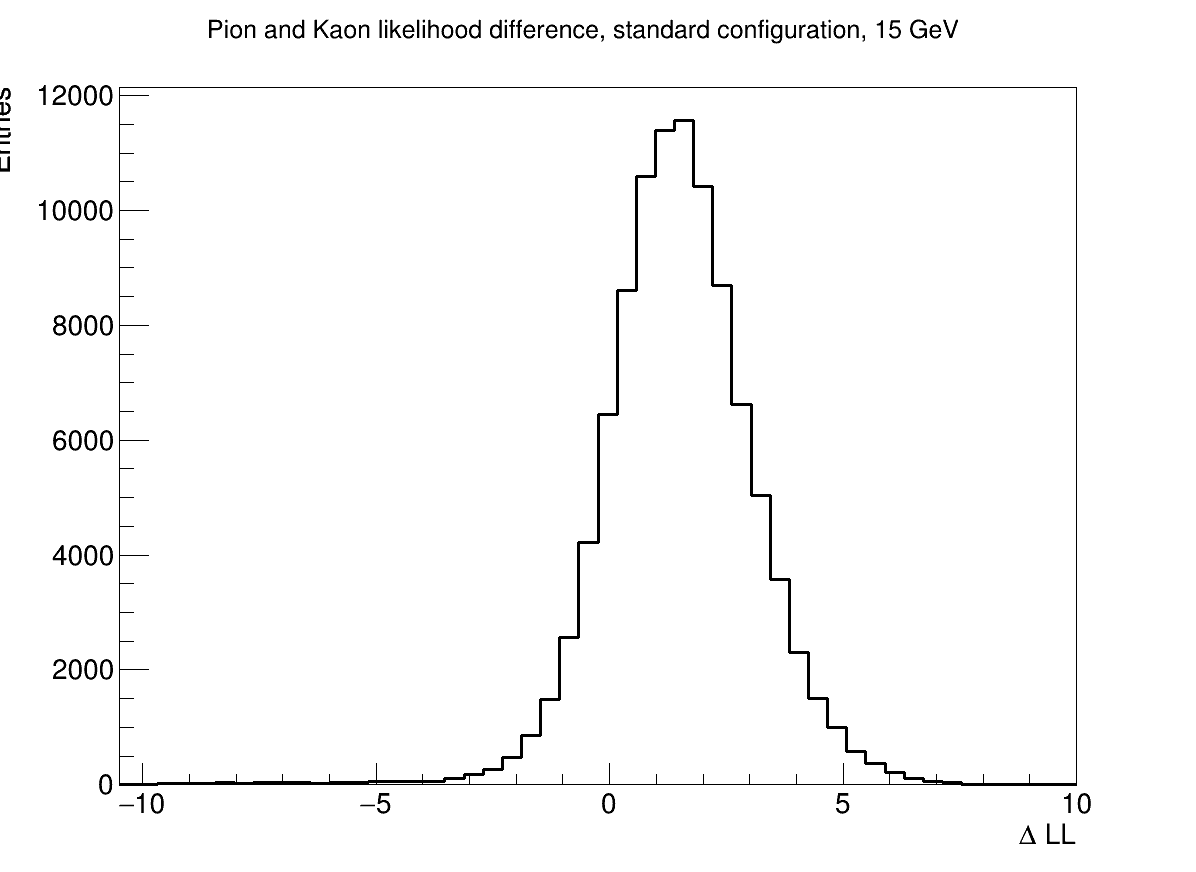
\includegraphics[width = 1.0\textwidth]{Plots/PionKaonDLL15GeVStandard.png}
      \caption{Pion-kaon $\Delta{\rm LL}$}
    \end{subfigure}
    \caption{Log likelihood at $\SI{15}{\giga\eV}$}
  \end{figure}
\end{frame}

\begin{frame}{Pion-Kaon likelihood simulations}
  \begin{figure}
    \centering
    \vspace{-0.2cm}
    \begin{subfigure}{0.5\textwidth}
      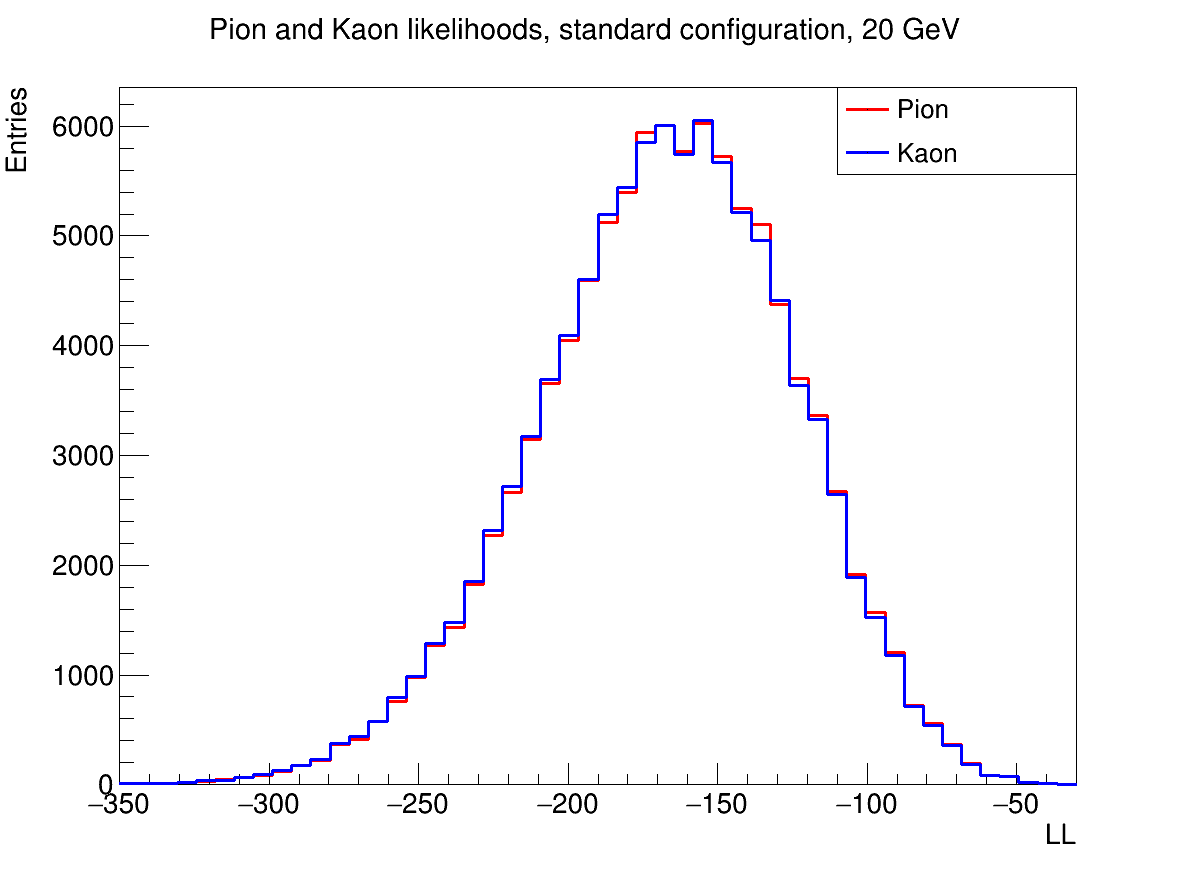
\includegraphics[width = 1.0\textwidth]{Plots/PionKaonLL20GeVStandard.png}
      \caption{Pion and kaon hypotheses}
    \end{subfigure}%
    \begin{subfigure}{0.5\textwidth}
      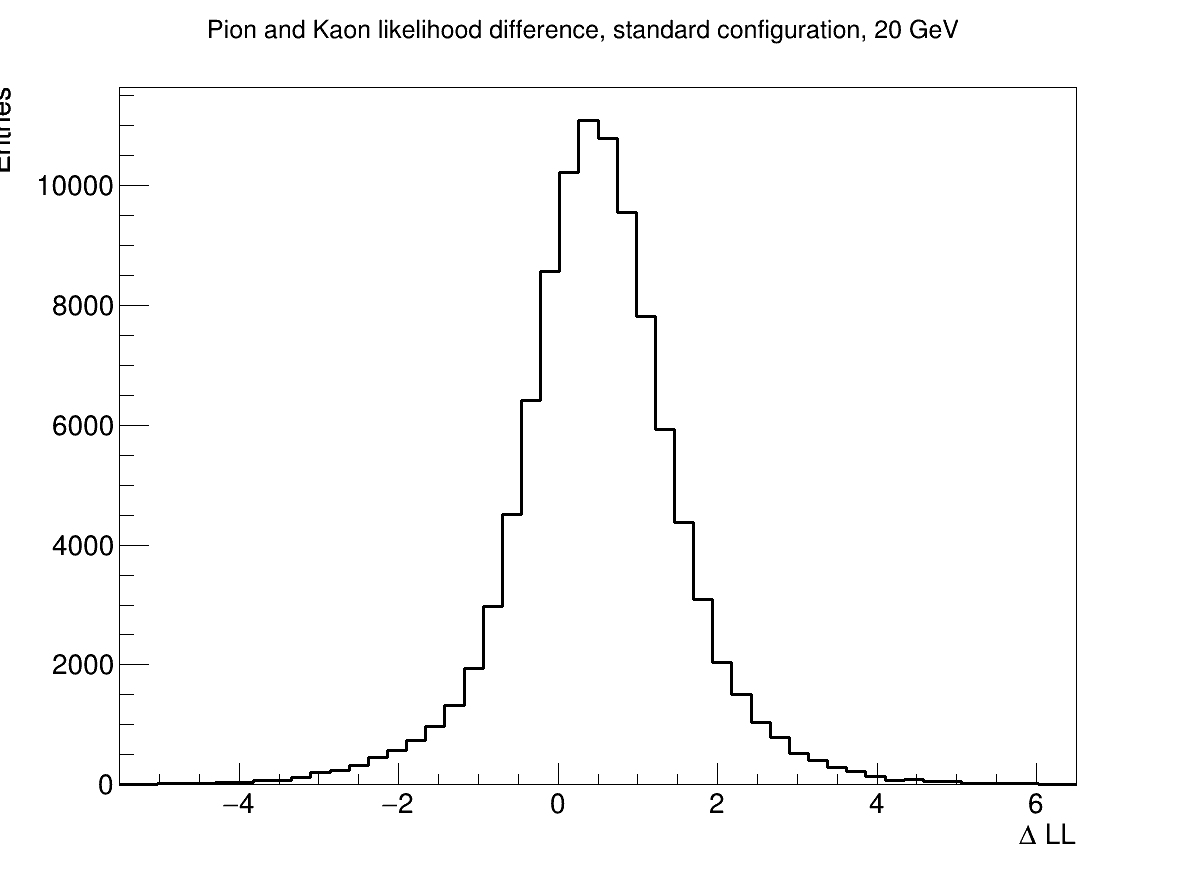
\includegraphics[width = 1.0\textwidth]{Plots/PionKaonDLL20GeVStandard.png}
      \caption{Pion-kaon $\Delta{\rm LL}$}
    \end{subfigure}
    \caption{Log likelihood at $\SI{20}{\giga\eV}$}
  \end{figure}
\end{frame}

\begin{frame}{Pion-Proton likelihood simulations}
  \begin{figure}
    \centering
    \vspace{-0.2cm}
    \begin{subfigure}{0.5\textwidth}
      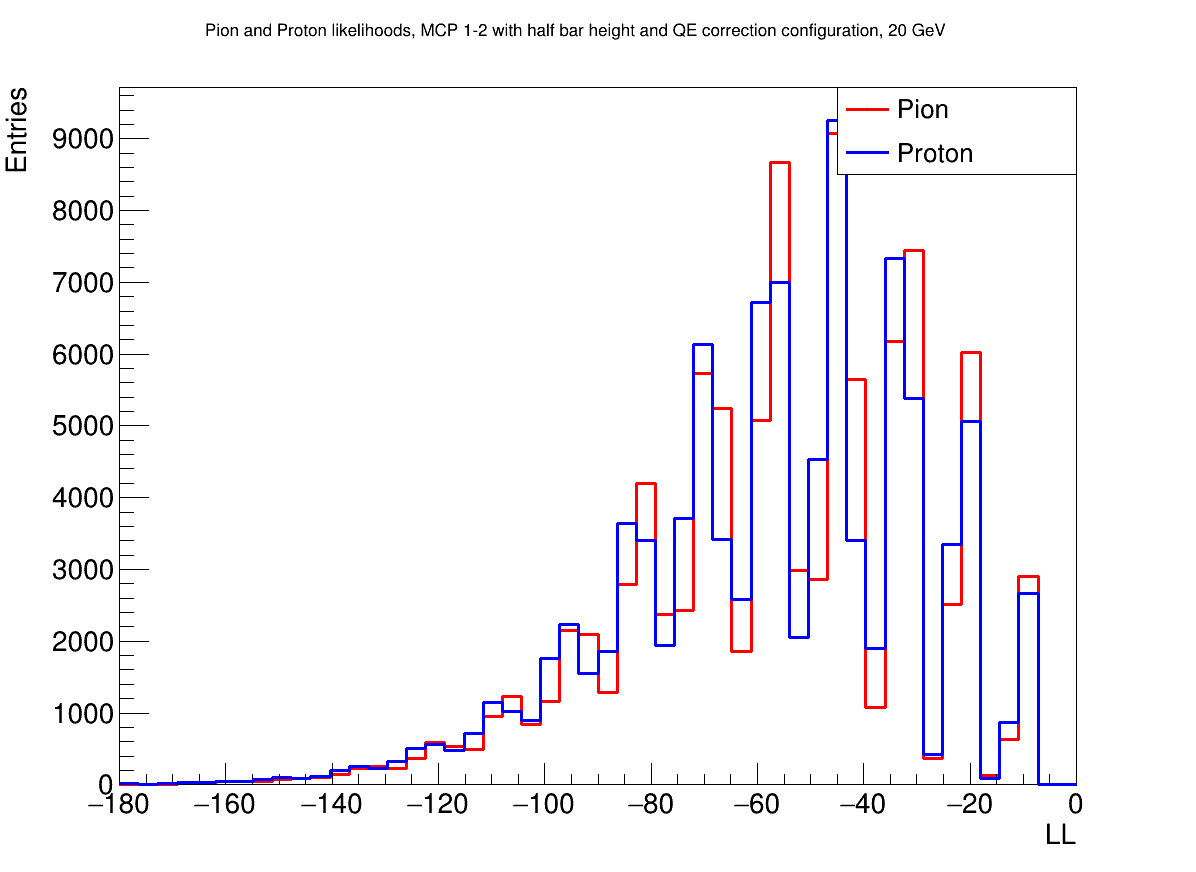
\includegraphics[width = 1.0\textwidth]{Plots/ProtonPionLL20GeVStandardMCPAB.png}
      \caption{Pion and proton hypotheses}
    \end{subfigure}%
    \begin{subfigure}{0.5\textwidth}
      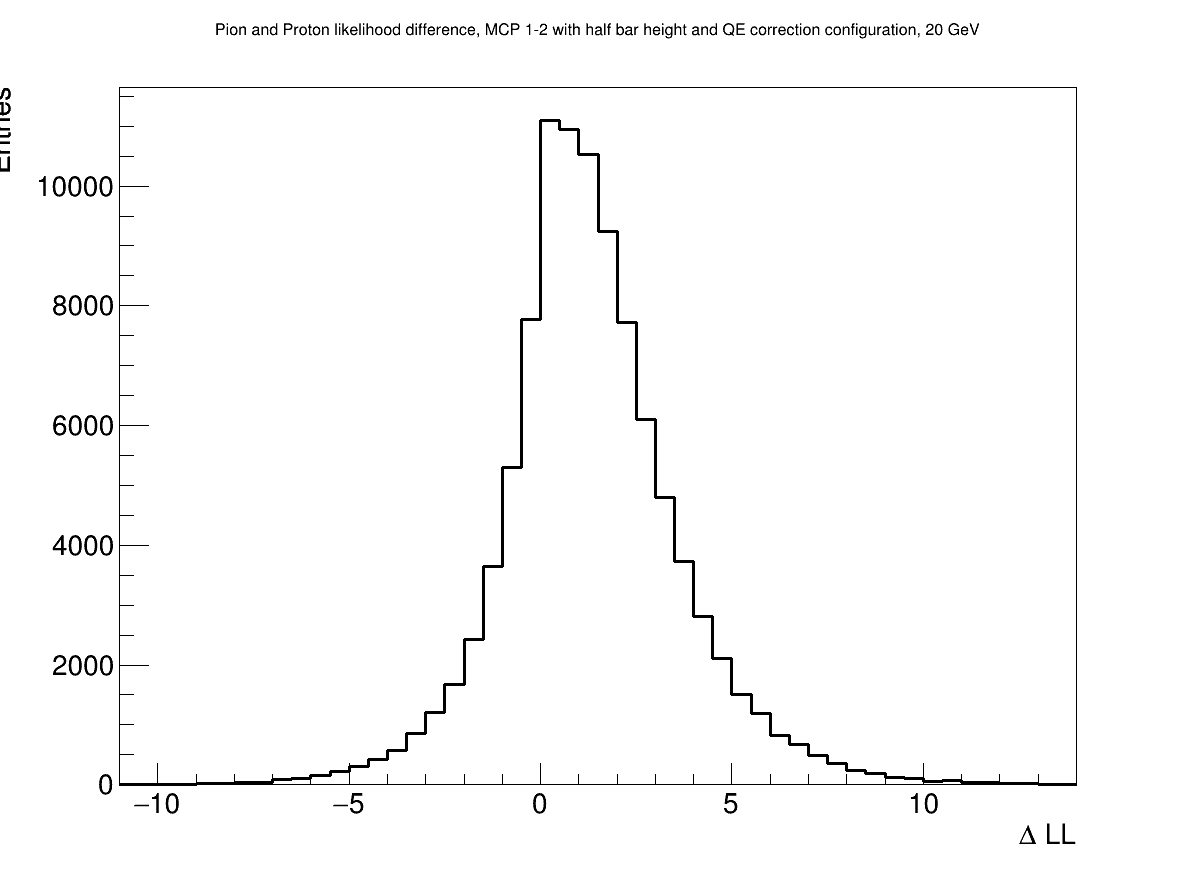
\includegraphics[width = 1.0\textwidth]{Plots/ProtonPionDLL20GeVStandardMCPAB.png}
      \caption{Pion-proton $\Delta{\rm LL}$}
    \end{subfigure}
    \caption{Log likelihood at $\SI{20}{\giga\eV}$}
  \end{figure}
  \begin{center}
    Adopt to testbeam setup: MCP A and B\\
    Assume MCP A has QE that is $65\%$ of MCP B
  \end{center}
\end{frame}

\begin{frame}{Pion-Kaon likelihood simulations}
  \begin{figure}
    \centering
    \vspace{-0.2cm}
    \begin{subfigure}{0.5\textwidth}
      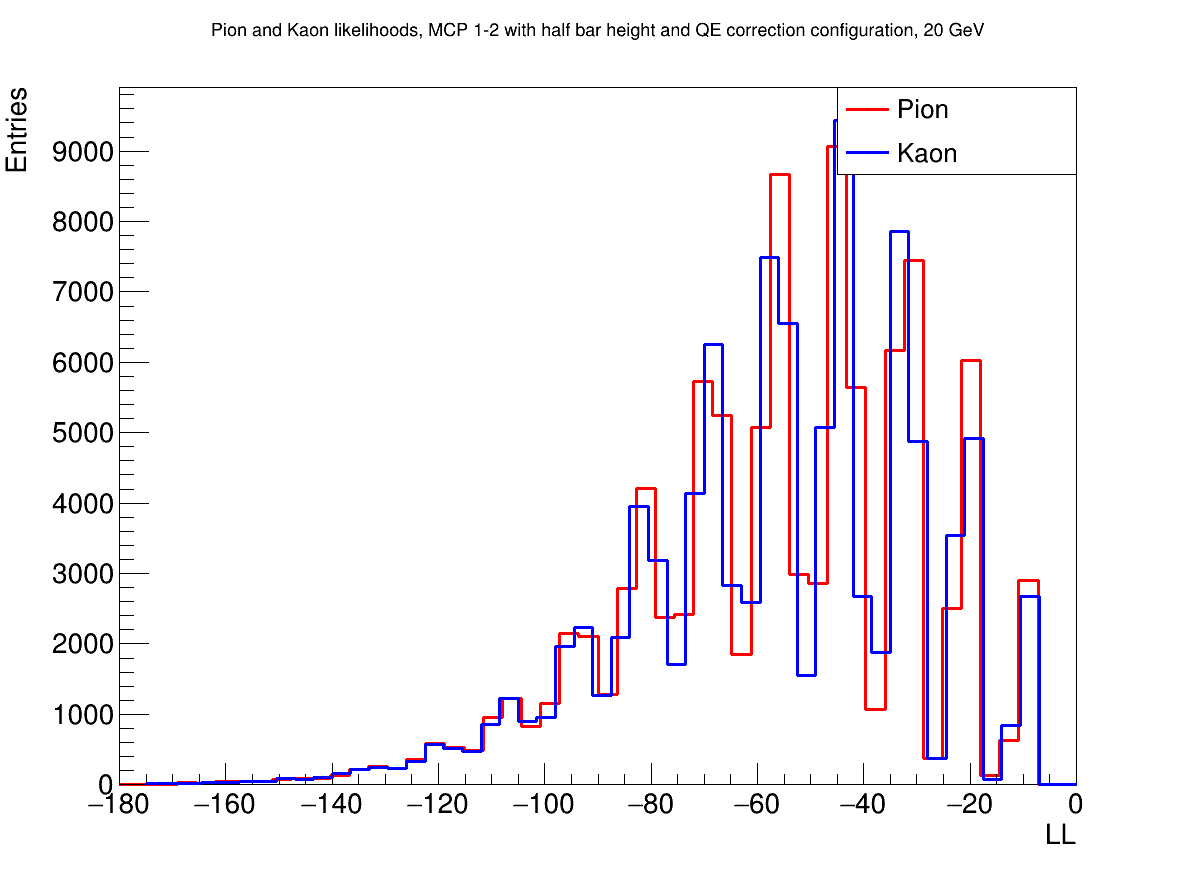
\includegraphics[width = 1.0\textwidth]{Plots/PionKaonLL20GeVStandardMCPAB.png}
      \caption{Pion and kaon hypotheses}
    \end{subfigure}%
    \begin{subfigure}{0.5\textwidth}
      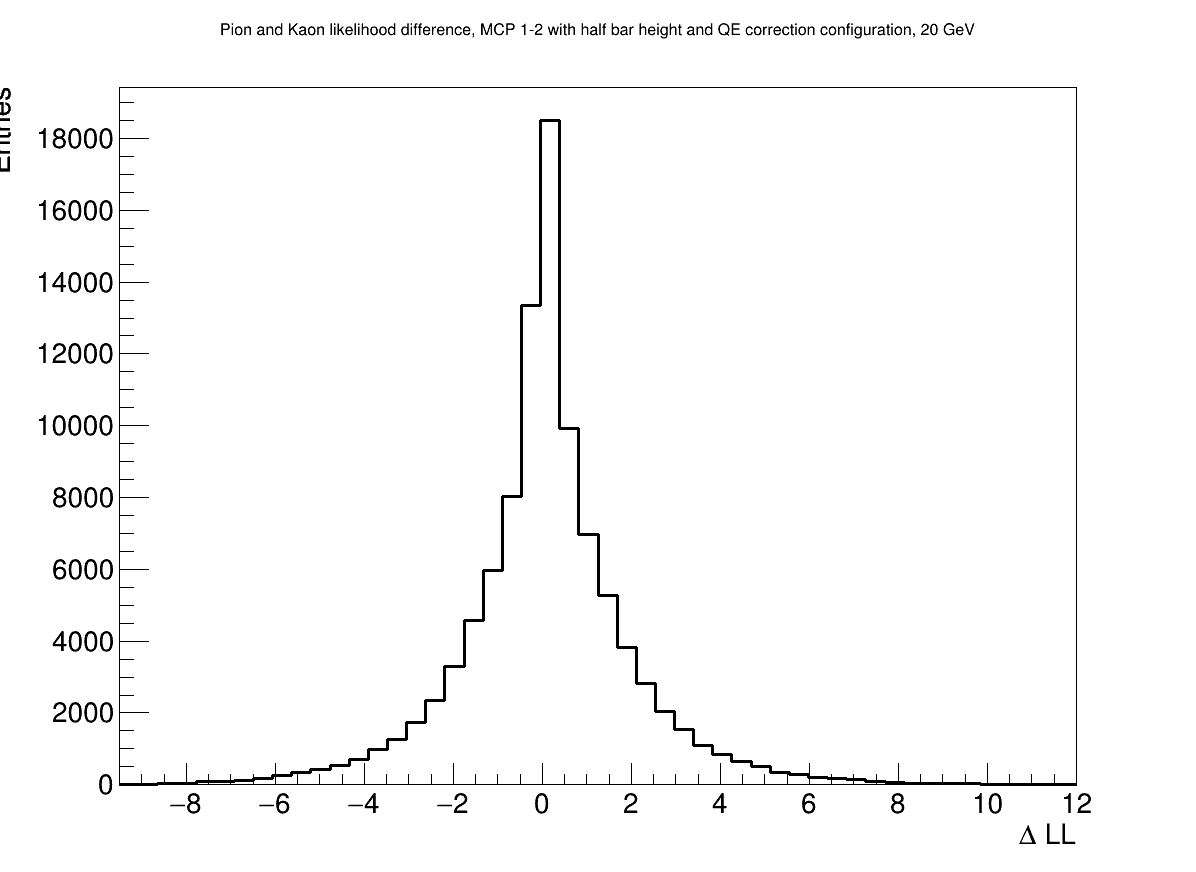
\includegraphics[width = 1.0\textwidth]{Plots/PionKaonDLL20GeVStandardMCPAB.png}
      \caption{Pion-kaon $\Delta{\rm LL}$}
    \end{subfigure}
    \caption{Log likelihood at $\SI{20}{\giga\eV}$}
  \end{figure}
  \begin{center}
    Adopt to testbeam setup: MCP A and B\\
    Assume MCP A has QE that is $65\%$ of MCP B
  \end{center}
\end{frame}

\section{PID efficiency studies}
\begin{frame}{PID efficiency from FTDR}
  \begin{center}
    PID efficiency study from FTDR \\
    Aim: Reproduce similar study with testbeam setup
  \end{center}
  \begin{figure}
    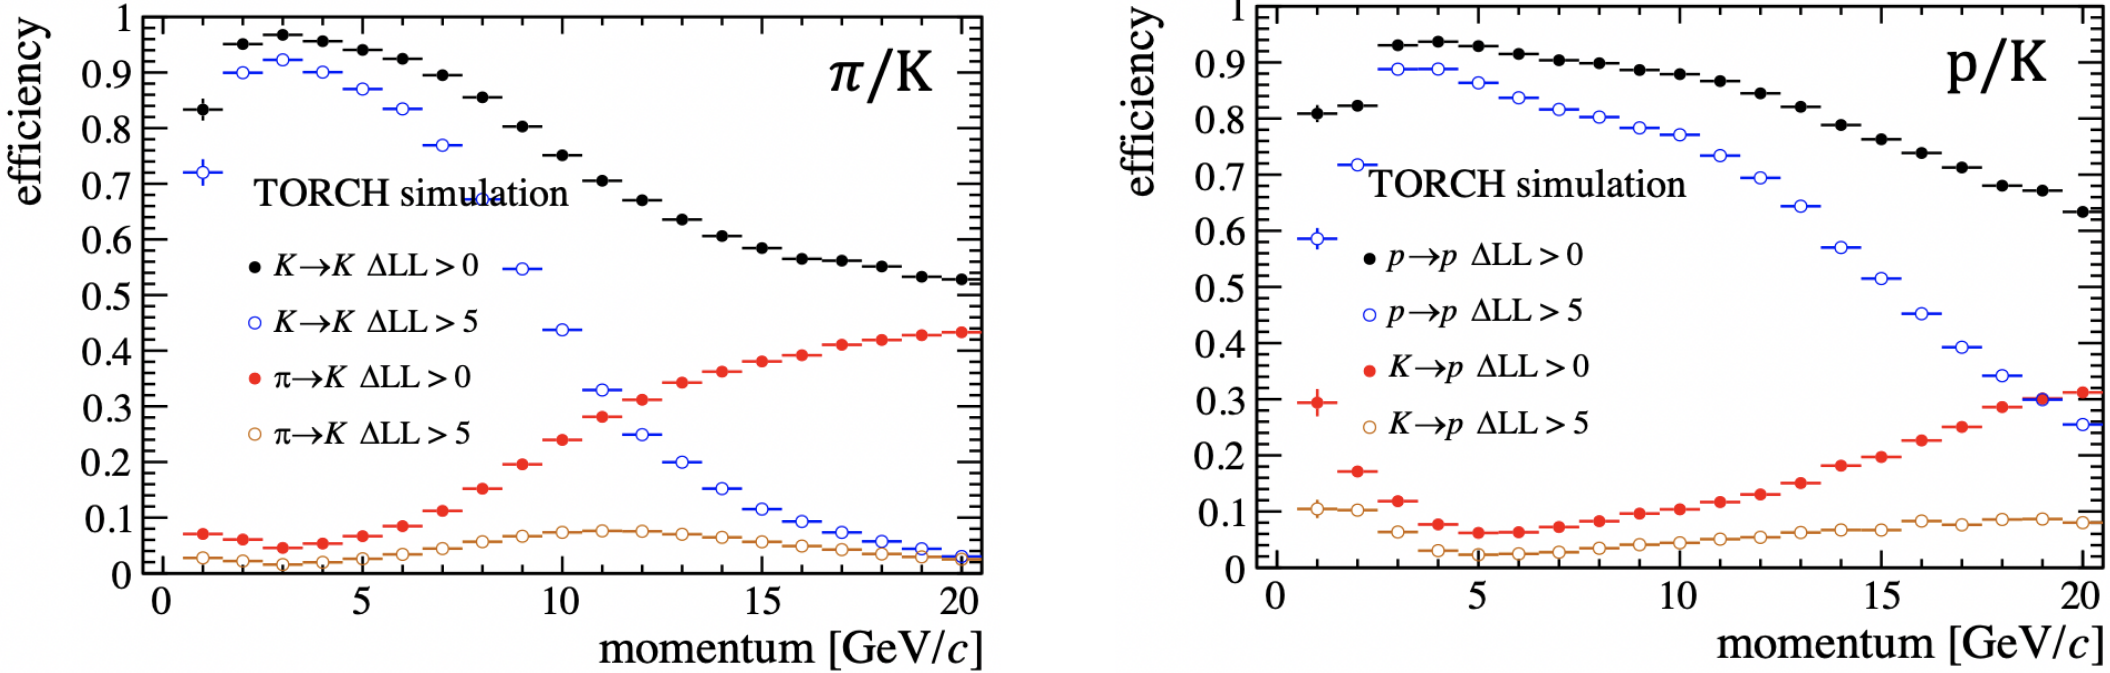
\includegraphics[width = 1.0\textwidth]{Plots/PIDEfficiencyFTDR.png}
  \end{figure}
\end{frame}

\begin{frame}{PID efficiency simulation}
  \begin{figure}
    \centering
    \vspace{-0.2cm}
    \begin{subfigure}{0.5\textwidth}
      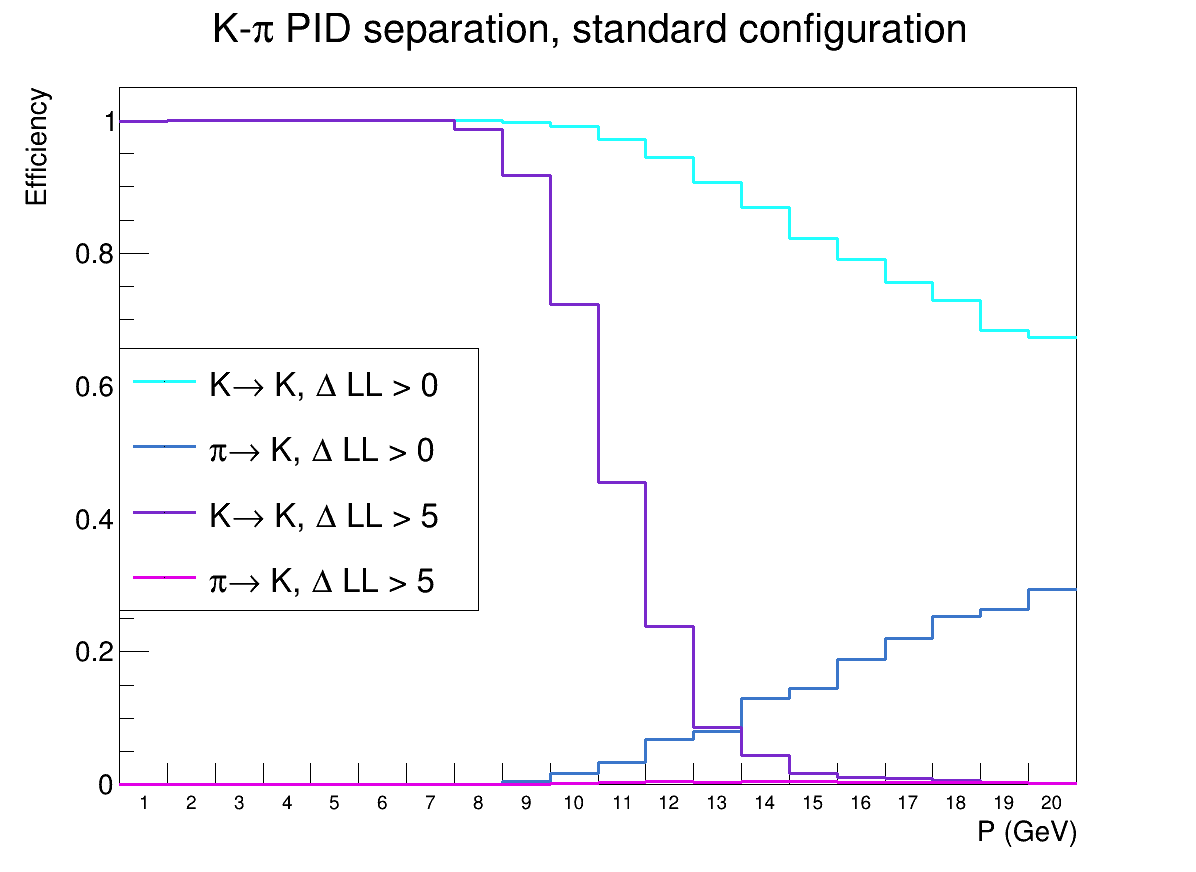
\includegraphics[width = 1.0\textwidth]{Plots/KaonPionPIDEfficiencyStandard.png}
      \caption{Kaon-pion}
    \end{subfigure}%
    \begin{subfigure}{0.5\textwidth}
      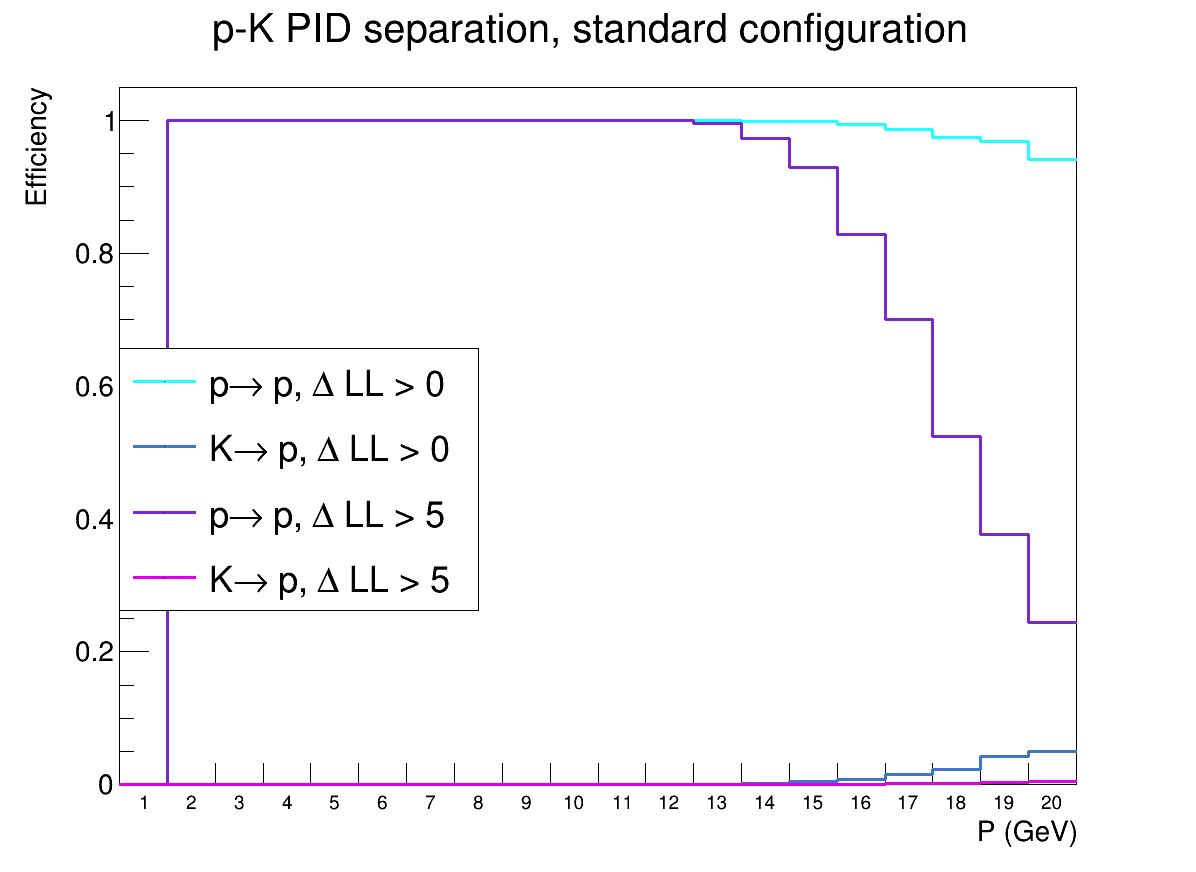
\includegraphics[width = 1.0\textwidth]{Plots/PionProtonPIDEfficiencyStandard.png}
      \caption{Pion-proton}
    \end{subfigure}
    \caption{PID efficiency}
  \end{figure}
  \begin{center}
    Full array of MCPs with same QE
  \end{center}
\end{frame}

\begin{frame}{PID efficiency simulation}
  \begin{figure}
    \centering
    \vspace{-0.2cm}
    \begin{subfigure}{0.5\textwidth}
      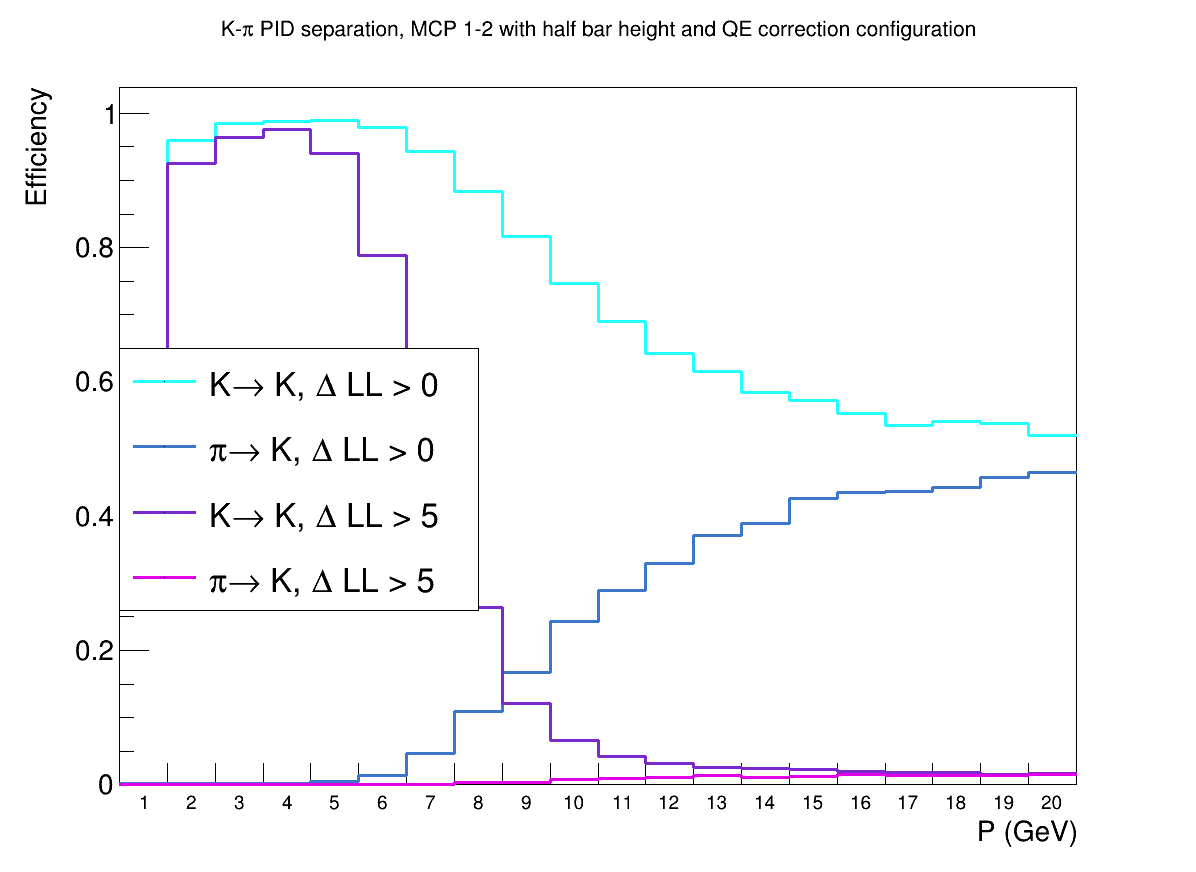
\includegraphics[width = 1.0\textwidth]{Plots/KaonPionPIDEfficiencyStandardMCPAB.png}
      \caption{Kaon-pion}
    \end{subfigure}%
    \begin{subfigure}{0.5\textwidth}
      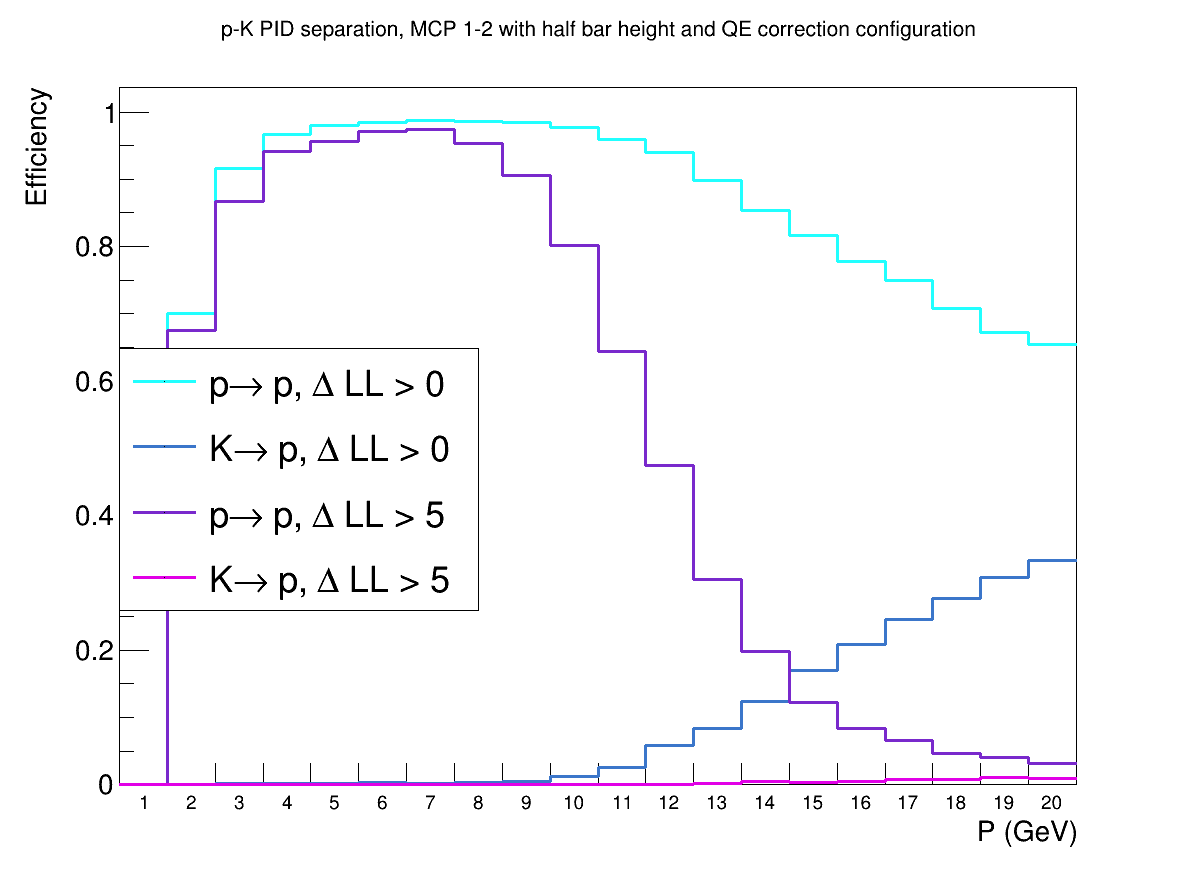
\includegraphics[width = 1.0\textwidth]{Plots/PionProtonPIDEfficiencyStandardMCPAB.png}
      \caption{Pion-proton}
    \end{subfigure}
    \caption{PID efficiency}
  \end{figure}
  \begin{center}
    2 MCPs, one with lower QE
  \end{center}
\end{frame}

\section{PID study of proto-TORCH testbeam data}
\begin{frame}{PID study of proto-TORCH testbeam data}
  Obviously, more messy and challenging:
  \begin{enumerate}
    \setlength\itemsep{1.0em}
    \item{Not many photons $\implies$ Use position 1 only}
    \item{Backgrounds $\implies$ For now, discard events where reconstruction fails}
    \begin{itemize}
      \item{Photon hits do not match track sometimes...}
    \end{itemize}
    \item{T2 has an unknown offset $\implies$ Align time distribution from simulation with that in data}
    \begin{itemize}
      \item{There is probably a much better way...}
    \end{itemize}
    \item{No T1 $\implies$ Introduce artificial $\SI{9500}{\milli\meter}$ offset to time information}
  \end{enumerate}
\end{frame}

\begin{frame}{Results from testbeam data}
  \begin{center}
    \begin{tabular}{lcccccc} 
      \hline
      PID cut                              & $\Delta{\rm LL} > 0$ & $\Delta{\rm LL} > 5$ \\
      \hline
      $\SI{8}{\giga\eV}$ pion simulation   & $99.0\%$             & $97.9\%$ \\
      $\SI{9}{\giga\eV}$ pion simulation   & $98.9\%$             & $96.8\%$ \\
      Proto-TORCH testbeam pions           & $78.6\%$             & $72.9\%$ \\
      \hline
      $\SI{8}{\giga\eV}$ proton simulation & $98.7\%$             & $97.4\%$ \\
      $\SI{9}{\giga\eV}$ proton simulation & $98.8\%$             & $96.5\%$ \\
      Proto-TORCH testbeam protons         & $66.9\%$             & $59.5\%$ \\
      \hline
    \end{tabular}
  \end{center}
\end{frame}

\section{Summary and next steps}
\begin{frame}{Summary and next steps}
  \begin{itemize}
    \setlength\itemsep{2.0em}
    \item{Summary}
    \begin{enumerate}
      \setlength\itemsep{1.0em}
      \item{Likelihood calculation gives consistent results}
      \item{Single particle simulation shows very good PID separation power}
      \item{Testbeam data show some PID separation power, but not as good as simulation}
    \end{enumerate}
    \item{Next steps:}
    \begin{enumerate}
      \setlength\itemsep{1.0em}
      \item{\color{red}Discuss with Neville!}
    \end{enumerate}
  \end{itemize}
\end{frame}

\end{document}
